\subsection{反交换代数与交错代数}

定义7. 一个Z型分次A-代数E称为反交换的，如果对所有非零齐次元素x，y\ensuremath{\in}E

\[
x y = (- 1) ^ {\deg (x) \deg (y)} y x.\tag{36}
\]

代数 \(\mathbf{E}\) 称为交错的，如果它是反交换的，并且还满足 \(x^{2} = 0\) （对每个奇次数的齐次元素 \(x\in \mathbf{E}\) ）。

注记. (1) 设 \(\mathbf{E}^{+}\) 为 \(\mathbf{E}\) 的分次子代数，即诸 \(\mathrm{E}_{2n}\) ( \(n \in \mathbf{Z}\) ) 的直和；由定义7可知，若 \(\mathbf{E}\) 是反交换的，则 \(\mathbf{E}^{+}\) 是包含在 \(\mathbf{E}\) 的中心（因而是交换的）中的子代数。

\begin{enumerate}
\def\labelenumi{(\arabic{enumi})}
\setcounter{enumi}{1}
\item
  假设2在E中不是零因子；那么若E是反交换的，则E是交错的，因为对于 \(x \in E\) 是奇次数的齐次元素这一情形，由(36)得 \(x^{2} = -x^{2}\) ，从而 \(2x^{2} = 0\) ，依假设即有 \(x^{2} = 0\) 。
\item
  我们将在 § 7 中详细研究交错代数的重要例子。
\end{enumerate}

引理4. 设E为Z型分次代数，S为一组齐次元素 \(\neq0\) ；E中所有齐次分量 \(x\neq0\) 均对每个 \(y\in S\) 满足关系式(36)的元素组成的集合F是E的分次子代数。

只需注意：(1) 如果 \(x'\) , \(x''\) 是两个次数同为 \(p\) 的齐次元素，\(y\) 是次数为 \(q\) 的齐次元素，并且 \(x'y = (-1)^{pq}yx'\) , \(x''y = (-1)^{pq}yx''\) ，那么也有 \((x' + x'')y = (-1)^{pq}y(x' + x'')\) ； (2) 若 \(x'\) , \(x''\) 是次数分别为 \(p'\) , \(p'', y\) 是次数为 \(q\) 的齐次元素，并且 \(x'y = (-1)^{p'q}yx'\) , \(x''y = (-1)^{p''q}yx''\) ，则

\[
(x ^ {\prime} x ^ {\prime \prime}) y = (- 1) ^ {(p ^ {\prime} + p ^ {\prime \prime}) q} y (x ^ {\prime} x ^ {\prime \prime}).
\]

命题13. 设 E 是类型为 Z 的分次 A-代数，且 S 是由代数 E 的非零齐次元素构成的一个生成系 \(\neq0\) ；为使 E 是反交换的（相应地，交错的），当且仅当 (36) 对所有 \(x\in S\) 和 \(y\in S\) 成立（相应地，该条件成立且进一步有：对所有属于S的奇次齐次元素x有 \(x^{2}=0\) ）。

我们首先考虑反交换代数的情形。根据引理4，由所有齐次分量 \(x \neq 0\) 均对所有 \(y \in S\) 满足 (36) 的元素构成的子代数F包含 S 的所有元素，因此 F = E。若现在 \(F'\) 类似地是 E 的这样的子代数：由所有齐次分量 \(x \neq 0\) 对每个非零齐次元素 \(y \neq 0\) 都满足 (36) 的元素组成，则由上述可知 \(F'\) 包含 S 的所有元素，因此 \(F' = E\) ，这就完成了命题在此情形下的证明。

为证明交错代数情形下的命题，可以假设 E 已经是反交换的；于是立即得出，E 中每个奇次数的齐次元素都具有形式 \(\sum_{i} z_{i} x_{i}\) ，其中 \(z_{i} \in E^{+}\) 且 \(x_{i} \in S\) 是奇次数的（利用 \(E^{+}\) 包含在 E 的中心中这一事实）；由此得出 \(\left(\sum_{i} z_{i} x_{i}\right)^{2} = \sum_{i} z_{i}^{2} x_{i}^{2} + \sum_{i < j} z_{i} z_{j} (x_{i} x_{j} + x_{j} x_{i}) = 0\) ，因为依假设有 \(x_{i}^{2} = 0\) ，且由 (36) 有 \(x_{i} x_{j} + x_{j} x_{i} = 0\) 。

命题 14. 设 E 和 F 是两个 Z 型分次 A-代数，均为反交换（相应地，交错）的。则斜张量积 \(\mathbf{E}^{\mathbf{g}}\otimes_{\mathbf{A}}\mathbf{F}\) （第 7 号）是一个反交换（相应地，交错）代数。

\(E^{g} \otimes_{A} F\) 的一个生成系由诸 \(x \otimes y\) 组成，其中 x（相应地，y）是 E（相应地，F）的齐次元素 \(\neq 0\) 。考虑这样两个元素 \(x \otimes y\) , \(x' \otimes y'\) ，其中 \(\deg(x) = p\) , \(\deg(y) = q\) , \(\deg(x') = p'\) , \(\deg(y') = q'\) ，使得 \(x \otimes y\) 的次数为 \(p + q\) ，而 \(x' \otimes y'\) 的次数为 \(p' + q'\) 。则由定义（第 7 号，公式 (27)）并由 (36)，

\[
(x \otimes y) (x ^ {\prime} \otimes y ^ {\prime}) = (- 1) ^ {q p ^ {\prime}} (x x ^ {\prime}) \otimes (y y ^ {\prime})
\]

\[
\begin{array}{r l} (x ^ {\prime} \otimes y ^ {\prime}) (x \otimes y) & = (- 1) ^ {p q ^ {\prime}} (x ^ {\prime} x) \otimes (y ^ {\prime} y) \\ & = (- 1) ^ {p q ^ {\prime} + p p ^ {\prime} + q q ^ {\prime}} (x x ^ {\prime}) \otimes (y y ^ {\prime}) \end{array}
\]

且命题 13 的判据表明 \(\mathbf{E}^{\mathbf{g}}\otimes_{\mathbf{A}}\mathbf{F}\) 是反交换的，因为 \(pq' + p p' + qq' - q p' \equiv (p + q)(p' + q')\) （模 2）。若进一步 E 和 F 是交错的且 \(p + q\) 是奇数，则数 \(p, q\) 中必有一个是奇数，因此 \((x \otimes y)^2 = \pm (x^2) \otimes (y^2) = 0\) 且命题 13 表明 \(E^g \otimes_A F\) 是交错的。

推论. 设 E 是一个 Z 型反交换（相应地，交错）分次 A-代数。则对每个环同态 \(\rho: \mathrm{A} \to \mathrm{B}\) ，分次 B-代数 \(\rho^{*}(\mathrm{E})\) （第 8 号，注 2）是反交换（相应地，交错）的。

环 B 配以平凡分次可视为一个交错 A-代数，且 \(\rho^{*}(\mathbf{E}) = \mathbf{E}^{\mathfrak{g}}\otimes_{\mathbf{A}}\mathbf{B}\) ，因此可应用命题 14。

注. 设 E 是一个 Z 型反交换分次 A-代数。则由 E 的乘法（§1，第 3 号）定义的从 \(E \otimes_{A} E\) 到 E 的 A-线性映射是分次 A-代数 \(E^{g} \otimes_{A} E\) 到 E 的同态，因为在命题 14 的记号下，在代数 E 中，

\[
(x y) (x ^ {\prime} y ^ {\prime}) = (- 1) ^ {q p ^ {\prime}} (x x ^ {\prime}) (y y ^ {\prime}).
\]

\section{张量代数，张量}

\subsection{模的张量代数的定义}

设 A 是一个交换环，M 是一个 A-模。对于每个整数 \(n \geqslant 0\) ，A-模，即 n 个都等于 M 的模的张量积（也称为 M 的第 n 次张量幂），记为 \(\bigotimes^{n} M\) ，或者 \(M^{\otimes n}\) ，或者 \(T^{n}(M)\) ，或者 \(T_{A}^{n}(M)\) ，或者 \(\operatorname{Tens}^{n}(M)\) ；于是 \(T^{1}(M) = M\) ；同时我们记 \(T^{0}(M) = A\) 。A-模，即直和 \(\bigoplus_{n \geqslant 0} T^{n}(M)\) ，记为 \(T(M)\) 或 \(\operatorname{Tens}(M)\) 。我们将在 \(T(M)\) 上定义一个类型为 N 的分次 A-代数结构，方法是：对每一对有序整数 \(p \geqslant 0\) , \(q \geqslant 0\) ，定义一个 A-线性映射

\[
m _ {p q} \colon \mathsf {T} ^ {p} (\mathbf {M}) \otimes_ {\mathbf {A}} \mathsf {T} ^ {q} (\mathbf {M}) \rightarrow \mathsf {T} ^ {p + q} (\mathbf {M})
\]

（§ 3，第 1 号，注记）。当 \(p > 0\) 且 \(q > 0\) 时， \(m_{pq}\) 是结合性同构（II，§ 3，第 9 号），而当 \(p = 0\) （相应地 \(q = 0\) ）时， \(m_{0,q}\) 是 \(A \otimes_A T^q(M)\) 到 \(T^q(M)\) 上的典范同构（相应地， \(m_{p,0}\) 是 \(T^p(M) \otimes_A A\) 到 \(T^p(M)\) 上的典范同构）（II，§ 3，第 4 号，命题 4）。然后，对于 \(x_t \in M\) , \(\alpha \in A\) ,

\[
\left\{ \begin{array}{r l} (x _ {1} \otimes \dots \otimes x _ {p}) \cdot (x _ {p + 1} \otimes \dots \otimes x _ {p + q}) & \\ = x _ {1} \otimes \dots \otimes x _ {p} \otimes x _ {p + 1} \otimes \dots \otimes x _ {p + q} \\ \alpha \cdot (x _ {1} \otimes \dots \otimes x _ {p}) = \alpha (x _ {1} \otimes \dots \otimes x _ {p}). \end{array} \right.\tag{1}
\]

显然，如此定义在 \(\mathsf{T}(\mathbf{M})\) 上的乘法满足结合律，并以单位元 \(1\) （即 \(\mathbf{A} = \mathsf{T}^0 (\mathbf{M})\) 的单位元）为单位元素。

定义1. 对于交换环A上的每个模M，M的张量代数，记为T(M)或Tens(M)，或 \(\mathsf{T}_{\mathbf{A}}(\mathbf{M})\) ，是代数 \(\bigoplus_{n\geqslant 0}\mathsf{T}^n (\mathbf{M})\) ，其乘法由(1)定义。典范单射 \(\phi :\mathsf{T}^{1}(\mathbf{M})\to \mathsf{T}(\mathbf{M})\) （II，§ 1，第 12 号）（也记作 \(\phi_{\mathbf{M}}\) ）称为M到T(M)的典范单射。

命题1. 设E是一个（含单位元的）A-代数，且 \(f:M\to E\) 为一个A-线性映射。存在唯一的一个A-代数同态 \(g:T(M)\to E\) ，使得 \(f=g\circ\phi\) .

换言之， \((\mathsf{T}(\mathbf{M}), \phi)\) 是泛映射问题（集合论，IV，§3，第1号）的一个解，其中 \(\Sigma\) 是A-代数结构的类， \(\alpha\) -映射是从模 M 到 A-代数的 A-线性映射。注意，这里完全不涉及 \(\mathsf{T}(\mathbf{M})\) 上的分次问题。

对于每个有限族 \((x_{i})_{1\leqslant i\leqslant n}\) ，它由 M 中的 n 个元素组成，根据 T(M) 中乘积的定义，有 \(x_{1}\otimes x_{2}\otimes\cdots\otimes x_{n}=\phi(x_{1})\phi(x_{2})\ldots\phi(x_{n})\) ；于是必然有 \(g(x_{1}\otimes x_{2}\otimes\cdots\otimes x_{n})=f(x_{1})f(x_{2})\ldots f(x_{n})\) （对 \(n\geqslant1\) ）且 \(g(\alpha)=\alpha e\) （若 e 是 E 的单位元）（对 \(\alpha\in A\) ），这就证明了 g 的唯一性。反之，注意到对所有 n\textgreater0，映射

\[
(x _ {1}, \dots , x _ {n}) \mapsto f (x _ {1}) f (x _ {2}) \dots f (x _ {n})
\]

从 \(\mathbf{M}^n\) 到 \(\mathbf{E}\) 的映射是 A-多重线性的；因此它对应着一个 A-线性映射 \(g_n: \mathsf{T}^n(\mathbf{M}) \to \mathbf{E}\) ，使得

\[
g \left(x _ {1} \otimes x _ {2} \otimes \dots \otimes x _ {n}\right) = f \left(x _ {1}\right) f \left(x _ {2}\right) \dots f \left(x _ {n}\right).\tag{2}
\]

我们还定义映射 \(g_0 \colon \mathsf{T}^0(\mathbf{M}) \to \mathbf{E}\) ，它等于 \(\eta_{\mathbf{E}}\) （§ 1，第 3 号），换言之， \(g_0(\alpha) = \alpha e\) （对 \(\alpha \in \mathbf{A}\) ）。设 \(g\) 是 \(\mathsf{T}(\mathbf{M})\) 到 \(\mathbf{E}\) 中的唯一的 A-线性映射，它在 \(\mathsf{T}^n(\mathbf{M})\) 上的限制为 \(g_n\) ( \(n \geqslant 0\) )；显然 \(g \circ \phi = g_1 = f\) ，剩下的只需验证 \(g\) 是 A-代数同态。由构造有 \(g(1) = e\) ，且由线性性只需证明 \(g(uv) = g(u)g(v)\) 对于 \(u \in \mathsf{T}^p(\mathbf{M})\) 和 \(v \in \mathsf{T}^q(\mathbf{M})\) ( \(p > 0, q > 0\) )成立；而现在由公式 (1) 和 (2) 可知，这一关系式当 \(u = x_1 \otimes x_2 \otimes \cdots \otimes x_p\) 且 \(v = x_{p+1} \otimes \cdots \otimes x_{p+q}\) （其中 \(x_i\) 属于 \(\mathbf{M}\) ）时成立。因此由线性性，它对于 \(u \in \mathsf{T}^p(\mathbf{M})\) 和 \(v \in \mathsf{T}^q(\mathbf{M})\) 成立。

注记。假设 \(\mathbf{E}\) 是类型为 \(\mathbf{Z}\) 的分次A-代数，其分次为 \((\mathbf{E}_n)\) ，并且还假设

\[
f (\mathbf {M}) \subset \mathrm{E} _ {1}.\tag{3}
\]

于是由(2)可知 \(g(\mathsf{T}^p (\mathbf{M})) \subset \mathrm{E}_p\) （对所有 \(p \geqslant 0\) ），因此 \(g\) 是分次代数同态。

\subsection{张量代数的函子性质}

命题2. 设A是一个交换环，M和N是两个A-模，且

\[
u: \mathbf {M} \rightarrow \mathbf {N}
\]

为一个A-线性映射。存在唯一一个A-代数同态

\[
u ^ {\prime}: \mathsf {T} (\mathbf {M}) \rightarrow \mathsf {T} (\mathbf {N})
\]

使得图表

\pandocbounded{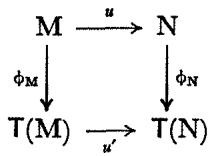
\includegraphics[keepaspectratio]{images/part003_fafbfb88.jpg}}

是可交换的。进一步地， \(u'\) 是分次代数同态。

存在性与唯一性 \(u'\) 由第 1 号命题 1 得出（把它应用于代数 \(T(N)\) 以及线性映射 \(\phi_N \circ u: M \to T(N)\) ）；由于

\[
u (\mathbf {M}) \subset \mathsf {T} ^ {1} (\mathbf {N}) = \mathbf {N},
\]

\(u'\) 是分次代数同态这一事实由第 1 号的注记得出。

命题 2 中的同态 \(u'\) 此后将记为 \(T(u)\) 。若 \(P\) 是一个 A-模，且 \(v: N \to P\) 是一个A-线性映射，则

\[
\mathsf {T} (v \circ u) = \mathsf {T} (v) \circ \mathsf {T} (u)\tag{4}
\]

因为 \(\mathsf{T}(v)\circ \mathsf{T}(u)\) 是使下图交换的代数同态

\pandocbounded{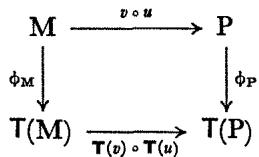
\includegraphics[keepaspectratio]{images/part003_f792dba1.jpg}}

\(\mathsf{T}(u)\) 有时称为 u 到 \(\mathsf{T}(\mathbf{M})\) （它包含 \(\mathbf{M} = \mathsf{T}^1(\mathbf{M})\) ）的典范扩张。注意，限制 \(\mathsf{T}^n(u): \mathsf{T}^n(\mathbf{M}) \to \mathsf{T}^n(\mathbf{N})\) 正是线性映射 \(u^{\otimes n} = u \otimes u \otimes \cdots \otimes u\) （n次），这由下式可知：

\[
\mathsf {T} ^ {n} (u) \left(x _ {1} \otimes \dots \otimes x _ {n}\right) = u \left(x _ {1}\right) \otimes \dots \otimes u \left(x _ {n}\right)
\]

因为 \(\mathsf{T}(u)\) 是一个代数同态且 \(\mathsf{T}^{1}(u)=u\) ；限制 \(\mathsf{T}^{0}(u)\) 在A上是恒等映射。 \(\mathsf{T}^{n}(u)\) 称为u的第n次张量幂。

命题3. 若 \(u: \mathbf{M} \to \mathbf{N}\) 是满射的A-线性映射，则同态 \(\mathsf{T}(u): \mathsf{T}(\mathbf{M}) \to \mathsf{T}(\mathbf{N})\) 是满射的，且其核是 \(\mathsf{T}(\mathbf{M})\) 的由核 \(\mathbf{P} \subset \mathbf{M} \subset \mathsf{T}(\mathbf{M})\) （即 \(u\) 的核）生成的双边理想。

\(T^{0}(u):T^{0}(M)\rightarrow T^{0}(N)\) 是双射的，且对每个整数 n\textgreater0,

\[
\mathbf {T} ^ {n} (u): \mathbf {T} ^ {n} (\mathbf {M}) \rightarrow \mathbf {T} ^ {n} (\mathbf {N})
\]

是满射的，这可通过对 \(n\) 作归纳并利用 II，§ 3，第 6 号，命题 6 看出；后一命题还表明（同样对 \(n\) 作归纳）， \(\mathfrak{S}_n\) （即 \(\mathsf{T}^n(u)\) 的核）是 \(\mathsf{T}^n(\mathbf{M})\) 中由乘积

\[
x _ {1} \otimes x _ {2} \otimes \dots \otimes x _ {n}
\]

生成，其中至少有一个 \(x_{i}\) 属于 \(\mathbf{P}\) 。这表明核 \(\mathfrak{S} = \bigoplus_{n\geqslant 1}\mathfrak{S}_n\) （即 \(\mathsf{T}(u)\) 的核）是由 \(\mathbf{P}\) 在 \(\mathsf{T}(\mathbf{M})\) 中生成的双边理想。

若 \(u: \mathbf{M} \to \mathbf{N}\) 是单射线性映射，则 \(\mathbf{T}(u)\) 并不总是单射映射（练习1）。然而，当 \(u\) 是使 \(u(\mathbf{M})\) 成为 \(\mathbf{N}\) 中直因子的单射时，结论成立，因为此时存在一个线性映射 \(v: \mathbf{N} \to \mathbf{M}\) ，使得 \(v \circ u\) 是 \(\mathbf{M}\) 上的恒等映射，从而

\[
\mathsf {T} (v \circ u) = \mathsf {T} (v) \circ \mathsf {T} (u)
\]

是 \(\mathsf{T}(\mathbf{M})\) 上的恒等映射，因此 \(\mathsf{T}(u)\) 是单射的，且其像（同构于 \(\mathsf{T}(\mathbf{M})\) ）是 \(\mathsf{T}(\mathbf{N})\) 的直因子（II，§1，第9号，命题15）。更精确地说：

命题4. 设N和P是A-模M的两个子模，使得它们的和 \(N + P\) 是M中的直因子，且它们的交 \(N \cap P\) 是N和P中的直因子。则同态 \(\mathsf{T}(\mathbf{N}) \to \mathsf{T}(\mathbf{M})\) , \(\mathsf{T}(\mathbf{P}) \to \mathsf{T}(\mathbf{M})\) 和

\[
\mathsf {T} (\mathbf {N} \cap \mathbf {P}) \rightarrow \mathsf {T} (\mathbf {M}),
\]

典范单射的典范扩张是单射；如果 \(\mathsf{T}(\mathbf{N})\) , \(\mathsf{T}(\mathbf{P})\) 和 \(\mathsf{T}(\mathbf{N} \cap \mathbf{P})\) 通过这些同态被等同于 \(\mathsf{T}(\mathbf{M})\) 的子代数，则

\[
\mathsf {T} (\mathbf {N} \cap \mathbf {P}) = \mathsf {T} (\mathbf {N}) \cap \mathsf {T} (\mathbf {P}).\tag{5}
\]

根据假设，存在子模 \(N' \subset N\) 和 \(P' \subset P\) ，使得 \(N = N' \oplus (N \cap P)\) , \(P = P' \oplus (N \cap P)\) ；于是

\[
\mathbf {N} + \mathbf {P} = \mathbf {N} ^ {\prime} \oplus \mathbf {P} ^ {\prime} \oplus (\mathbf {N} \cap \mathbf {P})
\]

并且根据假设存在子模 \(M'\) ⊂ M，使得

\[
\begin{array}{c} \mathbf {M} = \mathbf {M} ^ {\prime} \oplus (\mathbf {N} + \mathbf {P}) = \mathbf {M} ^ {\prime} \oplus \mathbf {N} ^ {\prime} \oplus \mathbf {P} ^ {\prime} \oplus (\mathbf {N} \cap \mathbf {P}) \\ = \mathbf {M} ^ {\prime} \oplus \mathbf {P} ^ {\prime} \oplus \mathbf {N} = \mathbf {M} ^ {\prime} \oplus \mathbf {N} ^ {\prime} \oplus \mathbf {P}. \end{array}
\]

特别地， \(N + P\) ，N，P以及 \(N \cap P\) 是M中的直因子，这（如前所述）意味着典范同态

\[
\begin{array}{l} \mathsf {T} (\mathbf {N} + \mathbf {P}) \to \mathsf {T} (\mathbf {M}), \qquad \mathsf {T} (\mathbf {N}) \to \mathsf {T} (\mathbf {M}), \\ \mathsf {T} (\mathbf {P}) \to \mathsf {T} (\mathbf {M}), \qquad \mathsf {T} (\mathbf {N} \cap \mathbf {P}) \to \mathsf {T} (\mathbf {M}) \end{array}
\]

是单射的。三个代数 \(\mathsf{T}(\mathbf{N})\) , \(\mathsf{T}(\mathbf{P})\) 和 \(\mathsf{T}(\mathbf{N} \cap \mathbf{P})\) 因此被等同于 \(\mathsf{T}(\mathbf{N} + \mathbf{P})\) 的子代数，而后者被等同于 \(\mathsf{T}(\mathbf{M})\) 的子代数；

记 \(\mathbf{Q} = \mathbf{N} \cap \mathbf{P}\) ，则只需证明：若 \(\mathsf{T}(\mathbf{Q})\) , \(\mathsf{T}(\mathbf{N}' \oplus \mathbf{Q})\) 和 \(\mathsf{T}(\mathbf{P}' \oplus \mathbf{Q})\) 通过这些同态被等同于 \(\mathsf{T}(\mathbf{N}' \oplus \mathbf{P}' \oplus \mathbf{Q})\) 的子代数，则

\[
\mathsf {T} (\mathbf {N} ^ {\prime} \oplus \mathbf {Q}) \cap \mathsf {T} (\mathbf {P} ^ {\prime} \oplus \mathbf {Q}) = \mathsf {T} (\mathbf {Q}).\tag{6}
\]

现在，考虑交换图

\pandocbounded{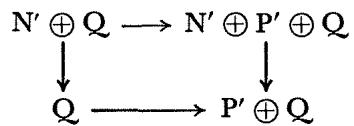
\includegraphics[keepaspectratio]{images/part003_8d12e188.jpg}}

其中水平箭头是典范单射，垂直箭头是典范投影。我们由此导出一个交换图

\begin{enumerate}
\def\labelenumi{(\arabic{enumi})}
\setcounter{enumi}{6}
\tightlist
\item
\end{enumerate}

\pandocbounded{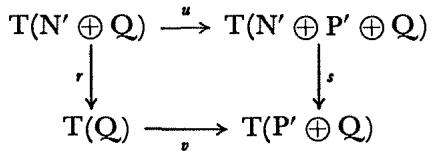
\includegraphics[keepaspectratio]{images/part003_389443db.jpg}}

其中 r 和 s 是满同态（命题 3），而 u 和 v 是单同态。因此，为证明 (6)，注意到右端显然包含于左端；于是只需验证：若

\[
x \in \mathsf {T} (\mathbf {N} ^ {\prime} \oplus \mathbf {Q}) \cap \mathsf {T} (\mathbf {P} ^ {\prime} \oplus \mathbf {Q}),
\]

那么 \(x \in \mathsf{T}(\mathsf{Q})\) 。现在，同态 s 的定义表明，它在 \(\mathsf{T}(\mathsf{P}' \oplus \mathsf{Q})\) （等同于 \(\mathsf{T}(\mathsf{N}' \oplus \mathsf{P}' \oplus \mathsf{Q})\) 的一个子代数）上的限制是恒等映射；因此关于 x 的假设蕴含 \(s(u(x)) = x\) 。但此时也有 \(v(r(x)) = x\) ，换言之，x 属于 \(\mathsf{T}(\mathsf{Q})\) 在 \(\mathsf{T}(\mathsf{P}' \oplus \mathsf{Q})\) 中的像，这就是要证明的。

注。特别地，当 A 是域时（II，§ 7，第 3 号，命题 4），命题 4 的假设对 M 的任意子模 N, P 总是成立。此外，若 N ⊂ P 且 N ≠ P，则对所有 n ≥ 1 有 T \(^{n}\) (N) ≠ T \(^{n}\) (P)，因为如果 R 是 P 在 N 中的补，则 T \(^{n}\) (P) ∩ T \(^{n}\) (R) = \{0\} 由(4)及T \(^{n}\) (R) ≠ \{0\}.

推论。设K是一个交换域，M是K上的一个向量空间。对于每一个元素 \(z \in \mathsf{T}(\mathbf{M})\) 存在一个M的最小子空间N，使得 \(z \in \mathsf{T}(\mathbf{N})\) 且N在K上具有有限秩。

在这个陈述中约定，对于 M 的每个向量子空间 P， \(T(P)\) 典范地等同于 \(T(M)\) 的一个子代数。设 \(z \in T(M)\) ；z 可以表示为一些元素的线性组合，其中每个元素都是 \(M = T^{1}(M)\) 中元素的有限乘积；出现在这些乘积中的 M 的所有元素生成一个有限秩的向量子空间 Q，且 \(z \in T(Q)\) .

设 \(\mathfrak{F}\) 为由有限秩向量子空间 \(\mathbf{P}\) （满足 \(z\in \mathsf{T}(\mathbf{P})\) ）组成的（非空）集合。 \(\mathfrak{F}\) 中元素的每个递减序列都是平稳的，因为它们是有限秩的向量空间。因此 \(\mathfrak{F}\) 有一个极小元素 \(\mathbf{N}\) （集合论，III，§6，第5号）。还需验证每个 \(\mathbf{P}\in \mathfrak{F}\) 包含 \(\mathbf{N}\) ；现在， \(z\in \mathsf{T}(\mathbf{P})\cap \mathsf{T}(\mathbf{N}) = \mathsf{T}(\mathbf{P}\cap \mathbf{N})\) （命题4）；根据 \(\mathbf{N}\) 的定义，这意味着 \(\mathbf{N}\cap \mathbf{P} = \mathbf{N}\) ，即 \(\mathbf{P}\supset \mathbf{N}\) .

M的子空间N称为与z相关联的。

\subsection{标量环的扩张}

设A，A'为两个交换环，且 \(\rho:A\to A'\) 为一个环同态。设M为一个A-模，M'为一个A'-模，且 \(u:M\to M'\) 为一个A-同态；由于典范单射 \(\phi_{M'}:M'\to T_{A'}(M')\) （通过标量限制）也是一个A-同态，所以复合映射 \(M\xrightarrow{u}M'\xrightarrow{\phi_{M'}}T_{A'}(M')\) 也是A-同态。由（第 2 号）导出一个 A-代数同态 \(T_{A}(M)\to\rho*(T_{A'}(M'))\) ，也记为 \(T(u):T_{A}(M)\to T_{A'}(M')\) ，它是使图表交换的唯一 A-同态。

\begin{enumerate}
\def\labelenumi{(\arabic{enumi})}
\setcounter{enumi}{7}
\tightlist
\item
\end{enumerate}

\pandocbounded{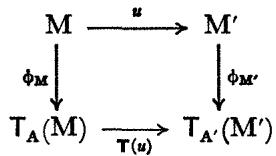
\includegraphics[keepaspectratio]{images/part003_9672ae23.jpg}}

若 \(\sigma: \mathbf{A}' \to \mathbf{A}''\) 是一个交换环同态， \(\mathbf{M}''\) 是一个 \(\mathbf{A}''\) -模，且 \(v: \mathbf{M}' \to \mathbf{M}''\) 是一个 \(\mathbf{A}'\) -同态，则上述唯一性性质表明

\[
\mathbf {T} (v \circ u) = \mathbf {T} (v) \circ \mathbf {T} (u).\tag{9}
\]

命题5. 设A，B为两个交换环， \(\rho: \mathbf{A} \to \mathbf{B}\) 一个环同态，且 M 是一个 A-模。典范扩张

\[
\psi : \mathsf {T} _ {\mathbf {B}} (\mathbf {B} \otimes_ {\mathbf {A}} \mathbf {M}) \rightarrow \mathbf {B} \otimes_ {\mathbf {A}} \mathsf {T} _ {\mathbf {A}} (\mathbf {M})
\]

（它是 B-线性映射 \(\mathbf{1}_{\mathbf{B}} \otimes \phi_{\mathbf{M}}: \mathbf{B} \otimes_{\mathbf{A}} \mathbf{M} \to \mathbf{B} \otimes_{\mathbf{A}} \mathsf{T}_{\mathbf{A}}(\mathbf{M})\) 的典范扩张）是分次 B-代数的同构。

考虑两个A-代数同态：典范单射 \(j: \mathbf{B} = \mathsf{T}^0(\mathbf{B} \otimes_{\mathbf{A}} \mathbf{M}) \to \mathsf{T}(\mathbf{B} \otimes_{\mathbf{A}} \mathbf{M})\) 及同态

\[
h = \mathsf {T} (i): \mathsf {T} (\mathbf {M}) \rightarrow \mathsf {T} (\mathbf {B} \otimes_ {\mathbf {A}} \mathbf {M})
\]

由典范 A-线性映射导出（参见公式 (8)），

\[
i: \mathbf {M} \rightarrow \mathbf {B} \otimes_ {\mathbf {A}} \mathbf {M}.
\]

由于 \(\mathsf{T}^0 (\mathbf{B}\otimes_{\mathbf{A}}\mathbf{M})\) 包含于 \(\mathsf{T}(\mathbf{B}\otimes_{\mathbf{A}}\mathbf{M})\) 的中心，可以应用 §4 第 2 号的命题 5，从而得到一个 A-代数同态

\[
\psi^ {\prime}: \mathbf {B} \otimes_ {\mathbf {A}} \mathsf {T} (\mathbf {M}) \rightarrow \mathsf {T} (\mathbf {B} \otimes_ {\mathbf {A}} \mathbf {M})
\]

，使得对于 \(\beta \in \mathbf{B}\) , \(x_{i} \in \mathbf{M}\) （ \(1 \leqslant i \leqslant n\) ），

\[
\psi^ {\prime} (\beta \otimes (x _ {1} \otimes x _ {2} \otimes \dots \otimes x _ {n})) = \beta ((1 \otimes x _ {1}) \otimes (1 \otimes x _ {2}) \otimes \dots \otimes (1 \otimes x _ {n})),
\]

这立即表明 \(\psi'\) 也是一个B-代数同态。只需证明 \(\psi \circ \psi'\) 和 \(\psi' \circ \psi\) 分别是 \(B \otimes_{A} T(M)\) 和 \(T(B \otimes_{A} M)\) 上的恒等映射。现在，这两个代数都由 \(B \otimes_{A} M\) 生成，并且显然 \(\psi \circ \psi'\) 和 \(\psi' \circ \psi\) 与 \(B \otimes_{A} M\) 上的恒等映射一致，由此得出结论。

\subsection{张量代数的正向极限}

设 \((\mathbf{A}_{\alpha},\phi_{\beta \alpha})\) 为一个交换环的有向正向系统，且 \((\mathbf{M}_{\alpha},f_{\beta \alpha})\) 为一个由 \(\mathbf{A}_{\alpha}\) -模构成的正向系统（II，§ 6，第 2 号）；设 \(\mathbf{A} = \varinjlim \mathbf{A}_{\alpha}\) 和 \(\mathbf{M} = \varinjlim \mathbf{M}_{\alpha}\) ，后者是一个 A-模。对于 \(\alpha \leqslant \beta\) ，一个 \(\mathbf{A}_{\alpha}\) -代数同态（第 3 号，公式 (8)） \(f_{\beta \alpha}' = \mathsf{T}(f_{\beta \alpha})\colon \mathsf{T}_{\mathbf{A}_{\alpha}}(\mathbf{M}_{\alpha})\to \mathsf{T}_{\mathbf{A}_{\beta}}(\mathbf{M}_{\beta})\) 由 \(\mathbf{A}_{\alpha}\) -同态 \(f_{\beta \alpha}\colon \mathbf{M}_{\alpha}\to \mathbf{M}_{\beta}\) 典范地导出，并且由（9）（第 3 号）可知 \((\mathsf{T}_{\mathbf{A}_{\alpha}}(\mathbf{M}_{\alpha}),f_{\beta \alpha}')\) 是一个由 \(\mathbf{A}_{\alpha}\) -代数构成的正向系统。另一方面，设 \(f_{\alpha}\colon \mathbf{M}_{\alpha}\to \mathbf{M}\) 为典范 \(\mathbf{A}_{\alpha}\) -同态；一个 \(\mathbf{A}_{\alpha}\) -代数同态 \(f_{\alpha}'\colon \mathsf{T}_{\mathbf{A}_{\alpha}}(\mathbf{M}_{\alpha})\to \mathsf{T}_{\mathbf{A}}(\mathbf{M})\) 由（第 3 号，公式 (8)）导出，并且由（9）（第 3 号）也可得出，诸 \(f_{\alpha}'\) 构成一个由 \(\mathbf{A}_{\alpha}\) -同态构成的正向系统。

命题6. A-同态 \(f' = \varinjlim f_{\alpha}' : \varinjlim T_{A_{\alpha}}(M_{\alpha}) \to T_{A}(M)\) 是一个分次代数同构。

为简化起见，我们记 \(\mathbf{E} = T_{\mathbf{A}}(\mathbf{M})\) 和 \(\mathbf{E}' = \varinjlim T_{\mathbf{A}_{\alpha}}(\mathbf{M}_{\alpha})\) ，并设

\[
g _ {\alpha}: \mathsf {T} _ {\mathrm{A} _ {\alpha}} (\mathbf {M} _ {\alpha}) \rightarrow \mathbf {E} ^ {\prime}
\]

为典范 \(\mathbf{A}_{\alpha}\) -同态。显然，复合 \(\mathbf{A}_{\alpha}\) -线性映射 \(\mathbf{M}_{\alpha} \xrightarrow{\phi_{\mathbf{M}_{\alpha}}} \mathsf{T}_{\mathbf{A}_{\alpha}}(\mathbf{M}_{\alpha}) \xrightarrow{g_{\alpha}} \mathbf{E}'\) 构成一个正向系统，因此存在唯一的 A-线性映射 \(u = \varinjlim (g_{\alpha} \circ \phi_{\mathbf{M}_{\alpha}}): \mathbf{M} \to \mathbf{E}'\) ，使得

\[
u \circ f _ {\alpha} = g _ {\alpha} \circ \phi_ {M _ {\alpha}}
\]

对所有 \(\alpha\) 成立。该映射本身唯一地分解（第 1 号，命题 1）为 \(\mathbf{M} \xrightarrow{\phi_{\mathbf{M}}} \mathrm{E} \to \mathrm{E}'\) ，其中 \(h\) 是一个 A-代数同态。只需证明 \(h \circ f' = 1_{\mathrm{E}'}\) 和 \(f' \circ h = 1_{\mathrm{E}}\) .

为此注意到，对于每个指标 \(\alpha\) （第3号，公式（8））

\[
h \circ f _ {\alpha} ^ {\prime} \circ \phi_ {M _ {\alpha}} = h \circ \phi_ {M} \circ f _ {\alpha} = u \circ f _ {\alpha} = g _ {\alpha} \circ \phi_ {M _ {\alpha}}
\]

由此，根据第1号命题1的唯一性断言，

\[
h \circ f _ {\alpha} ^ {\prime} = g _ {\alpha}
\]

对所有 \(\alpha\) 成立；由此可得 \((h \circ f') \circ g_{\alpha} = g_{\alpha}\) 对所有 \(\alpha\) 成立，因此由正向极限的定义得 \(h \circ f' = 1_{\mathbf{E}'}\) 。

另一方面，根据第3号公式（8），

\[
f ^ {\prime} \circ u \circ f _ {\alpha} = f ^ {\prime} \circ g _ {\alpha} \circ \phi_ {M _ {\alpha}} = f _ {\alpha} ^ {\prime} \circ \phi_ {M _ {\alpha}} = \phi_ {M} \circ f _ {\alpha},
\]

由此再次得到 \(f' \circ u = \phi_{\mathbb{M}}\) （由正向极限的定义）；我们得出 \(f' \circ h \circ \phi_{\mathbb{M}} = \phi_{\mathbb{M}}\) ，而第 1 号命题 1 的唯一性性质给出 \(f' \circ h = 1_{\mathbb{E}}\) .

命题6也可以通过观察以下事实来证明：对于每个整数 \(n \geqslant 1\) ，存在一个典范的 A-模同构 \(\lim_{\longrightarrow} \mathsf{T}_{\mathbf{A}_{\alpha}}^{n}(\mathbf{M}_{\alpha}) \to \mathsf{T}_{\mathbf{A}}^{n}(\mathbf{M})\) ，这由 II，§6，第3号，命题7通过对 \(n\) 作归纳得到。立即可验证，这些同构都是 \(f'\) 的限制。

\subsection{直和的张量代数。自由模的张量代数。分次模的张量代数。}

设 A 是一个交换环，且 \(M = \bigoplus_{\lambda \in L} M_{\lambda}\) 是一族A-模的直和。由II，§3，第7号，命题7，通过对n归纳可知， \(T^{n}(M)\) 是子模的直和，这些子模是典范单射的像

\[
\mathbf {M} _ {\lambda_ {1}} \otimes \mathbf {M} _ {\lambda_ {2}} \otimes \dots \otimes \mathbf {M} _ {\lambda_ {n}} \rightarrow \mathsf {T} ^ {n} (\mathbf {M}) = \mathbf {M} ^ {\otimes n}
\]

相对于所有序列 \((\lambda_{i})\in\mathbf{L}^{n}\) 。将 \(M_{\lambda_{1}}\otimes M_{\lambda_{2}}\otimes\cdots\otimes M_{\lambda_{n}}\) 与这个像等同，可以看出 \(T(\mathbf{M})\) 是下列模的直和

\[
\mathbf {M} _ {\lambda_ {1}} \otimes \mathbf {M} _ {\lambda_ {2}} \otimes \dots \otimes \mathbf {M} _ {\lambda_ {n}}
\]

（其中 \(n\) 遍历 \(\mathbf{N}\) ，且对每个 \(n\) ， \((\lambda_t)\) 遍历 \(\mathbf{L}^n\) .

我们首先推导出以下结论：

定理1. 设A为交换环，M为自由A-模，且 \((e_{\lambda})_{\lambda \in L}\) 为 M 的一组基。则诸元素 \(e_{s} = e_{\lambda_{1}} \otimes e_{\lambda_{2}} \otimes \cdots \otimes e_{\lambda_{n}}\) ——其中 \(s = (\lambda_{1}, \ldots, \lambda_{n})\) 遍历 L 中元素的所有有限序列的集合，而 \(e_{\varnothing}\) 用来表示 T(M) 的单位元——构成 A-模 T(M) 的一组基。

该基的元素显然是齐次的，且乘法表由下式给出

\[
e _ {s} e _ {t} = e _ {s t}\tag{10}
\]

（其中 \(st\) 表示由 \(\mathbf{L}\) 中元素组成的、通过并置序列 \(s\) 和 \(t\) 而得到的序列（I，§7，第2号）。

可以看出，T(M) 的基 \((e_{s})\) 连同乘法法则 (10) 典范同构于集合 L 上的自由幺半群（I，§7，第2号），该同构通过把这个幺半群的每个字 s 映到元素 \(e_{s}\) 而得到。由此（§2，第7号）可知，自由模 M（其基的指标集为 L）的张量代数 T(M) 典范同构于 L 在 A 上的自由结合代数。特别地（§2，第7号，命题7），对于每个从 L 到 A-代数 E 的映射 \(f: L \to E\) ，存在唯一的 A-代数同态 \(\bar{f}: T(M) \to E\) ，使得 \(\bar{f}(e_{\lambda}) = f(\lambda)\) 。

注。上述结果同样可以由自由结合代数和张量代数的泛性质推出，利用II，§3，第7号，命题7的推论2。

推论. 若 M 是投射 A-模，则 T(M) 是投射 A-模。

M 是自由 A-模 N 的一个直因子（II，§2，第 2 号，命题 4），因此 T(M) 是 T(N) 的一个直因子（第 2 号）；由于 T(N) 是自由的（定理 1），这表明 T(M) 是投射的（II，§2，第 2 号）。

命题7. 设 \(\Delta\) 是一个交换幺半群， \(\mathbf{M}\) 是一个 \(\Delta\) 型分次 A-模，而 \((\mathbf{M}_{\alpha})_{\alpha \in \Delta}\) 是其分次。对于每个有序对 \((\alpha, n) \in \Delta \times \mathbf{N}\) ，设 \(\mathsf{T}^{\alpha,n}(\mathbf{M})\) 为诸子模 \(\mathbf{M}_{\alpha_1} \otimes \mathbf{M}_{\alpha_2} \otimes \dots \otimes \mathbf{M}_{\alpha_n}\) （属于 \(\mathsf{T}^n(\mathbf{M})\) ，满足 \(\sum_{i=1}^{n} \alpha_i = \alpha\) ）的（直）和；于是 \((T^{\alpha, n}(M))_{(\alpha, n) \in \Delta \times N}\) 是唯一的 \(\Delta \times N\) 型分次，它与 \(T(M)\) 上的代数结构相容、并在 \(M = T^1(M)\) 上诱导出给定的分次。

在本号开头已经看到， \(\mathsf{T}(\mathbf{M})\) 是诸 \(\mathsf{T}^{\alpha,n}(\mathbf{M})\) 的直和，而这是一个与代数结构相容的分次这一事实直接由定义得出。若 \((\mathsf{T}'^{\alpha,n})\) 是另一个 \(\Delta \times \mathbf{N}\) 型分次，它在 \(\mathsf{T}(\mathbf{M})\) 上与代数结构相容且满足 \(\mathsf{T}^{\alpha,1}(\mathbf{M}) = \mathsf{T}'^{\alpha,1}\) （对 \(\alpha \in \Delta\) ），则直接由定义可知，对所有 \(n \geqslant 1\) 以及所有 \(\alpha \in \Delta\) ，有 \(\mathsf{T}^{\alpha,n}(\mathbf{M}) \subset \mathsf{T}'^{\alpha,n}\) ；但由于 \(\mathsf{T}(\mathbf{M})\) 也是诸 \(\mathsf{T}^{\alpha,n}(\mathbf{M})\) 的直和，这意味着 \(\mathsf{T}'^{\alpha,n} = \mathsf{T}^{\alpha,n}(\mathbf{M})\) (II，§1，第8号，注记)。

\subsection{张量与张量记号}

设 A 是一个交换环，M 是一个 A-模， \(\mathbf{M}^*\) 为 M 的对偶（II，§2，第3号），I 和 J 为两个不相交的有限集；A-模 \(\bigotimes_{i\in \mathrm{I}\cup \mathrm{J}}\mathbf{E}_i\) （其中 \(\mathbf{E}_i = \mathbf{M}\) （若 \(i\in \mathrm{I}\) ）， \(\mathbf{E}_i = \mathbf{M}^*\) （若 \(i\in \mathrm{J}\) ））记作 \(\mathsf{T}_{\mathsf{J}}^{\mathsf{I}}(\mathbf{M})\) ； \(\mathsf{T}_{\mathsf{J}}^{\mathsf{I}}(\mathbf{M})\) 的元素称为 M 上的 (I,J) 型张量。当 \(\mathbf{J} = \varnothing\) 时它们称为反变张量，当 \(\mathbf{I} = \varnothing\) 时称为协变张量，其余情形称为混合张量。

设 \(I'\) , \(I''\) 为 I 的两个子集，且 \(J'\) , \(J''\) 为 J 的两个子集，使得 \(I' \cup I'' = I\) , \(\mathbf{I}' \cap \mathbf{I}'' = \varnothing, \mathbf{J}' \cup \mathbf{J}'' = \mathbf{J}, \mathbf{J}' \cap \mathbf{J}'' = \varnothing\) ；则存在一个典范的结合同构（II，§3，第9号）

\[
\mathsf {T} _ {\mathbf {J}} ^ {\mathbf {I}} (\mathbf {M}) \rightarrow \mathsf {T} _ {\mathbf {J} ^ {\prime}} ^ {\mathbf {I} ^ {\prime}} (\mathbf {M}) \otimes_ {\mathbf {A}} \mathsf {T} _ {\mathbf {J} ^ {\prime \prime}} ^ {\mathbf {I} ^ {\prime \prime}} (\mathbf {M}).\tag{11}
\]

考虑张量代数 \(\mathsf{T}(\mathbf{M}\oplus \mathbf{M}^{*})\) ，由第 5 号可知 \(\mathsf{T}^n (\mathbf{M}\oplus \mathbf{M}^*)\) 典范地等同于诸 \(\mathsf{T}_{\mathbf{J}}^{\mathbf{I}}(\mathbf{M})\) 的直和，其中 I 遍历区间 \([1,n]\) （在 \(\mathbf{N}\) 中）的子集组成的集合，而 J 是 I 在 \([1,n]\) 中的补集。

当 \(I = [1, p]\) 且 \(J = [p + 1, p + q]\) ，其中整数 \(p \geqslant 0\) , \(q \geqslant 0\) （我们将 I（相应地 J）替换为 \(\varnothing\) ，如果 \(p = 0\) （相应地 \(q = 0\) ）），A-模 \(T_J^I(M)\) 也记作 \(T_q^p(M)\) ；A-模 \(T_0^n(M)\) 和 \(T_n^0(M)\) 根据定义分别是 A-模 \(T^n(M)\) 和 \(T^n(M^*)\) 。当 I 和 J 是基数为 \(p = \text{Card}(I)\) 和 \(q = \text{Card}(J)\) 的任意有限集合时，我们给它们每一个赋予一个全序；那么存在一个从 I（相应地 J）到 \([1, p]\) （相应地 \([p + 1, p + q]\) ）上的递增双射，因此这些双射定义了一个同构

\[
\mathbf {T} _ {\mathrm{J}} ^ {\mathrm{I}} (\mathbf {M}) \rightarrow \mathbf {T} _ {q} ^ {p} (\mathbf {M}).
\]

当 M 是有限生成的投射 A-模时，由 II，§ 2，第 7 号，命题 13 的推论 4 以及 II，§ 4，第 4 号，命题 4 的推论 1 可知，存在一个典范同构

\[
(\mathsf {T} _ {\mathbf {J}} ^ {\mathbf {I}} (\mathbf {M})) ^ {*} \to \mathsf {T} _ {\mathbf {I}} ^ {\mathbf {J}} (\mathbf {M}).
\]

现在假设 \(\mathbf{M}\) 是一个有限生成的自由 A-模，且设 \((e_{\lambda})_{\lambda \in L}\) 为 \(\mathbf{M}\) 的一组基（因此 L 是有限集）。 \(\mathbf{M}^*\) 的与 \((e_{\lambda})\) 对偶的基（II，§2，第 6 号）记为 \((e^{\lambda})_{\lambda \in L}\) 。基 \((e_{\lambda})\) 和 \((e^{\lambda})\) （分别属于 \(\mathbf{M}\) 和 \(\mathbf{M}^*\) ）定义了（第 5 号） \(\mathsf{T}_{\mathbf{J}}^{\mathbf{I}}(\mathbf{M})\) 的一个基，我们明确给出如下：给定两个映射 \(f\colon \mathbf{I} \to \mathbf{L}\) 和 \(g\colon \mathbf{J} \to \mathbf{L}\) ，设 \(e_f^g\) 为元素 \(\bigotimes_{i \in I \cup J} x_i\) （属于 \(\mathsf{T}_{\mathbf{J}}^{\mathbf{I}}(\mathbf{M})\) ），定义为

\[
x _ {i} = e _ {f (i)} \quad \text { if } i \in \mathbf {I}, \qquad x _ {i} = e ^ {g (i)} \quad \text { if } i \in \mathbf {J}.
\]

当 \((f, g)\) 遍历映射 \(f: \mathbf{I} \to \mathbf{L}\) 和 \(g: \mathbf{J} \to \mathbf{L}\) 的有序对组成的集合时，诸 \(e_f^g\) 构成 A-模 \(\mathsf{T}_{\mathbf{J}}^{\mathbf{I}}(\mathbf{M})\) 的一组基，称为与给定基 \((e_{\lambda})\) （ \(\mathbf{M}\) 的）相关联的基。对于 \(z \in \mathsf{T}_{\mathbf{J}}^{\mathbf{I}}(\mathbf{M})\) ，我们因此可以写出

\[
z = \sum_ {(f, g)} \alpha_ {g} ^ {f} (z). e _ {f} ^ {g}\tag{12}
\]

其中 \(\alpha_g^f\) 是关于基 \((e_f^g)\) 的坐标线性型；按照语言的约定俗成， \(\alpha_g^f(z)\) 称为张量 \(z\) 关于模 M 的基 \((e_\lambda)\) 的坐标。诸 \(\alpha_g^f\) 构成 \((e_g^f)\) 的对偶基，换言之，它们与 \(\mathsf{T}_{\mathbf{I}}^{\mathbf{j}}(\mathbf{M})\) 的基的元素等同，该基与 \((e_\lambda)\) 相关联。当 I 和 J 是 N 中区间 \([1,n]\) 的互补子集时， \(\alpha_g^f\) （或 \(\alpha_g^f(z)\) ）记法如下：每个元素 \(f(i)\) （对于 \(i\in I\) ）写作第 \(i\) 位上的上标，并在第 \(i\) 位处放一个点（对 \(i \in \mathbf{J}\) ）；类似地， \(g(i)\) （对于 \(i \in \mathbf{J}\) ）写作第 \(i\) 位上的下标，并在第 \(i\) 位处放一个点（对 \(i \in \mathbf{I}\) ）。例如，对于 \(\mathbf{I} = \{1, 4\}\) , \(\mathbf{J} = \{2, 3\}\) ，我们记 \(\alpha_{\cdot \nu \rho}^{\lambda \cdot \cdot \mu}\) ，如果 \(f(1) = \lambda, f(4) = \mu, g(2) = \nu, g(3) = \rho\) 。

设 \((\bar{e}_{\lambda})_{\lambda \in L}\) 为 M 的另一组基，且 \(P\) 为从 \((e_{\lambda})\) 到 \((\bar{e}_{\lambda})\) 的过渡矩阵（II，§ 10，第 8 号）。则从 \((e^{\lambda})\) 到 \((\bar{e}^{\lambda})\) （ \((\bar{e}_{\lambda}))\) 的对偶基）的过渡矩阵是 \(^{t}P^{-1}\) ，即 \(P\) 的逆步（II，§ 10，第 8 号，命题 5）。由此可得（II，§ 10，第 10 号），从基 \((e_{f}^{g})\) （属于 \(\mathrm{T}_{\mathrm{J}}^{\mathrm{I}}(\mathrm{M})\) ）到基 \((\bar{e}_{f}^{g})\) (其中 \(f\) （相应地 \(g\) ) 遍历从 I 到 L（相应地，从 J 到 L）的映射集合）的过渡矩阵是矩阵

\[
\bigotimes_ {i \in I \cup J} Q _ {i}, \quad \text { where } Q _ {i} = P \text { if } i \in I, Q _ {i} = ^ {t} P ^ {- 1} \text { if } i \in J.\tag{13}
\]

因此，该矩阵的转置被等同于

\[
\bigotimes_ {i \in \mathbf {I} \cup J} R _ {i}, \quad \text { where } R _ {i} = ^ {t} P ^ {- 1} \text { if } i \in \mathbf {I}, R _ {i} = P \text { if } i \in \mathbf {J}.\tag{14}
\]

现在假设 \(\mathbf{M}\) 是任意模。设 \(i\in \mathbf{I}, j\in \mathbf{J}\) 并记 \(\mathbf{I}' = \mathbf{I} - \{i\}, J' = J - \{j\}\) ；我们将定义一个典范的 A-线性映射

\[
c _ {j} ^ {i} \colon \mathsf {T} _ {\mathbf {J}} ^ {\mathbf {I}} (\mathbf {M}) \to \mathsf {T} _ {\mathbf {J} ^ {\prime}} ^ {\mathbf {I} ^ {\prime}} (\mathbf {M}),
\]

称为指标 \(i\) 与指标 \(j\) 的缩并。为此，注意到 \(\mathbf{M}^{\mathrm{I}} \times (\mathbf{M}^{*})^{\mathrm{J}}\) 上的映射，它将每个族 \((x_{i})_{i \in \mathbf{I} \cup \mathbf{J}}\) （其中 \(x_{i} \in \mathbf{M}\) （若 \(i \in \mathbf{I}\) ）， \(x_{i} \in \mathbf{M}^{*}\) （若 \(i \in \mathbf{J}\) ））对应到元素

\[
\left\langle x _ {i}, x _ {j} \right\rangle \otimes_ {k \in (\mathbb {I} \cup \mathbb {J}) - \{i, j \}} x _ {k}\tag{15}
\]

（属于 \(T_{J'}^{I'}(M)\) ）是 A-多重线性的； \(c_{j}^{i}\) 是对应的 A-线性映射。

现在假设 M 是自由且有限生成的，并令 \((e_{\lambda})_{\lambda \in L}\) 为 M 的一组基。给定两个映射 \(f: I \to L\) , \(g: J \to L\) ，设 \(f_i\) 表示 f 在 \(I' = I - \{i\}\) 上的限制， \(g_j\) 表示 g 在 \(J' = J - \{j\}\) 上的限制；于是根据 (12)

\[
c _ {j} ^ {i} (e _ {f} ^ {g}) = \left\{ \begin{array}{l l} 0 & \text { if } f (i) \neq g (j) \\ e _ {f _ {i}} ^ {g _ {j}} & \text { if } f (i) = g (j) \end{array} \right.\tag{16}
\]

\(c_j^i(z)\) 的坐标作为 \(z\) 的坐标的函数的表达式由此得出；对于每个映射 \(f'\) （相应地 \(g'\) ）——从 \(I'\) 到 \(L\) （相应地，从 \(J'\) 到 \(L\) ）——以及每个 \(\lambda \in L\) ，设 \((f', \lambda)\) （相应地 \((g', \lambda)\) ）表示从 \(I\) 到 \(L\) （相应地，从 \(J\) 到 \(L\) ）的、在 \(I'\) （相应地 \(J'\) ）上的限制为 \(f'\) （相应地 \(g'\) ）、并且以 \(\lambda\) 为其在元素 \(i\) （相应地 \(j\) ）处的值的映射。那么，若关于基 \((e_{f'}^{g'})\) （ \(T_{J'}^{I'}(M)\) 的基）的坐标线性型记为 \(\beta_{g'}^{f'}\) ,

\[
\beta_ {g ^ {\prime}} ^ {f ^ {\prime}} (c _ {j} ^ {i} (z)) = \sum_ {\lambda \in L} \alpha_ {(g ^ {\prime}, \lambda)} ^ {(f ^ {\prime}, \lambda)} (z).\tag{17}
\]

张量的例子。(1) 设 M 是有限生成的投射 A-模。我们知道（II，§ 4，第 2 号，命题 2 的推论），存在一个典范的 A-模同构

\[
\theta_ {\mathbf {M}} \colon \mathbf {M} ^ {*} \otimes_ {\mathbf {A}} \mathbf {M} \rightarrow \operatorname{End} _ {\mathbf {A}} (\mathbf {M})
\]

，使得 \(\theta_{\mathbf{M}}(x^{*}\otimes x)\) （对于 \(x\in \mathbf{M},x^{*}\in \mathbf{M}^{*}\) ）是自同态

\[
y \mapsto \langle y, x ^ {*} \rangle x.
\]

因此，借助 \(\theta_{\mathbf{M}}\) , \(\mathsf{T}_{(1)}^{(2)}(\mathbf{M})\) （同构于 \(\mathsf{T}_1^1 (\mathbf{M}))\) 可与 A-模 \(\operatorname{End}_{\mathbf{A}}(\mathbf{M})\) 等同。假设 \(\mathbf{M}\) 是自由模，且设 \((e_{\lambda})_{\lambda \in \mathbf{L}}\) 为 \(\mathbf{M}\) 的一组基；那么张量 \(z\in \mathbf{M}^*\otimes \mathbf{M}\) 关于该模的基 \((e^{\mu}\otimes e_{\lambda})\) 的坐标记为 \(\zeta_{\mu}^{\cdot \lambda}\) 。由于 \(\theta_{\mathrm{M}}(e^{\mu}\otimes e_{\lambda})\) 是自同态 \(y\mapsto \langle y,e^{\mu}\rangle e_{\lambda}\) ，自同态 \(u = \theta_{\mathrm{M}}(z) = \theta_{\mathrm{M}}\left(\sum_{\lambda ,\mu}\zeta_{\mu}^{\cdot \lambda}e^{\mu}\otimes e_{\lambda}\right)\) 把 \(y\) 映到 \(\sum_{\lambda ,\mu}\zeta_{\mu}^{\cdot \lambda}\langle y,e^{\mu}\rangle e_{\lambda}\) ；取 \(y = e_{\lambda}\) ，我们得到关系式

\[
u (e _ {\lambda}) = \sum_ {\mu \in L} \zeta_ {\lambda} ^ {\cdot \mu} e _ {\mu}\tag{18}
\]

换言之，线性映射 \(u = \theta_{\mathrm{M}}(z)\) 的矩阵是这样的矩阵：其位于指标 \(\mu\) 的行与指标 \(\lambda\) 的列交叉处的元素为 \(\zeta_{\lambda}^{\mu}\) 。

\(u\) 的迹的定义（II，§4，第3号）立即表明

\[
\operatorname{Tr} (\theta_ {\mathbb {M}} (z)) = c _ {1} ^ {2} (z).
\]

因此，元素 \(z_0 = \sum_{\lambda \in L} e^\lambda \otimes e_\lambda\) （其坐标 \(\zeta_\mu^{\cdot \lambda}\) 对于 \(\lambda \neq \mu\) 为零，对于 \(\lambda = \mu\) 等于1），它满足 \(\theta_M(z_0) = 1_M\) ，是元素 \(1 \in A = T_0^0(M)\) 在映射（缩并的转置）下的像。

\[
c _ {1} ^ {2}: \mathbf {T} _ {\{1 \}} ^ {\{2 \}} (\mathbf {M}) \rightarrow \mathbf {A}.
\]

\begin{enumerate}
\def\labelenumi{(\arabic{enumi})}
\setcounter{enumi}{1}
\tightlist
\item
  始终假设 M 是有限生成的投射 A-模；存在一个典范的 A-模同构
\end{enumerate}

\[
\mu : \mathbf {M} ^ {*} \otimes_ {\mathbf {A}} \mathbf {M} ^ {*} \rightarrow (\mathbf {M} \otimes_ {\mathbf {A}} \mathbf {M}) ^ {*}
\]

（II，§4，第 4 号，命题 2 的推论 1）以及一个典范同构

\[
\theta : (\mathbf {M} \otimes_ {\mathbf {A}} \mathbf {M}) ^ {*} \otimes_ {\mathbf {A}} \mathbf {M} \rightarrow \operatorname{Hom} _ {\mathbf {A}} (\mathbf {M} \otimes_ {\mathbf {A}} \mathbf {M}, \mathbf {M})
\]

（II，§4，第 2 号，命题 2 的推论）；此外 \(\operatorname{Hom}_{\mathbf{A}}(\mathbf{M} \otimes_{\mathbf{A}} \mathbf{M}, \mathbf{M})\) 典范同构于 A-模 \(\mathcal{L}_2(\mathbf{M}, \mathbf{M}; \mathbf{M})\) ，即由从 \(\mathbf{M} \times \mathbf{M}\) 到 \(\mathbf{M}\) 的 A-双线性映射组成的模（II，§3，第 9 号）。复合这些同构，得到典范同构

\[
\chi_ {\mathbf {M}} \colon T _ {\{1, 2 \}} ^ {(3)} (\mathbf {M}) = \mathbf {M} ^ {*} \otimes \mathbf {M} ^ {*} \otimes \mathbf {M} \rightarrow \mathcal {L} _ {2} (\mathbf {M}, \mathbf {M}; \mathbf {M})
\]

使得，对于 \(x^{*}, y^{*}\) （属于 \(\mathbf{M}^{*}\) ）， \(z \in \mathbf{M}\) ， \(\chi_{\mathbf{M}}(x^{*} \otimes y^{*} \otimes z)\) 是双线性映射

\[
(u, v) \mapsto \langle u, x ^ {*} \rangle \langle v, y ^ {*} \rangle z.
\]

因此，借助 \(\chi_{\mathbf{M}}\) , \(\mathsf{T}_{\{1,2\}}^{(3)}(\mathbf{M})\) （同构于 \(\mathsf{T}_{2}^{1}(\mathbf{M})\) ）可与 A-模 \(\mathcal{L}_2(\mathbf{M},\mathbf{M};\mathbf{M})\) 等同。假设 \(\mathbf{M}\) 是一个自由 A-模，且设 \((e_{\lambda})_{\lambda \in L}\) 为 \(\mathbf{M}\) 的一组基；那么张量 \(z\in \mathbf{M}^*\otimes \mathbf{M}^*\otimes \mathbf{M}\) 关于该模的基 \((e^{\lambda}\otimes e^{\mu}\otimes e_{\nu})\) 的坐标记为 \(\zeta_{\lambda \mu}^{\cdot \cdot \nu}\) 。双线性映射 \(\chi_{\mathbf{M}}(z)\) 把有序对 \((e_{\lambda},e_{\mu})\) 映到

\[
\sum_ {\nu \in L} \zeta_ {\lambda \mu}^{\cdot \cdot \nu} e _ {\nu}
\]

因此诸 \(\zeta_{\lambda \mu}^{\cdots \nu}\) 正是定义在 \(\mathbf{M}\) 上、由双线性映射 \(\chi_{\mathbf{M}}(z)\) 给出的（一般非结合的）代数关于基 \((e_{\lambda})\) 的结构常数（ \(\S 1\) ，第 7 号）。

注记2. 设 \((e_{\lambda})_{\lambda \in L}, (\tilde{e}_{\lambda})_{\lambda \in L}\) 为 M 的两个基，且 \(P\) 为从 \((e_{\lambda})\) 到 \((\tilde{e}_{\lambda})\) 的过渡矩阵。根据例1中所见， \(P\) 中位于指标 \(\lambda\) 的行与指标 \(\mu\) 的列交叉处的元素记为 \(\alpha_{\mu}^{\lambda}\) ，逆步 \(^{t}P^{-1}\) 中位于指标 \(\lambda\) 的行与指标 \(\mu\) 的列交叉处的元素记为 \(\beta_{\lambda}^{\mu}\) 。于是（采用上面引入的记号）

\begin{enumerate}
\def\labelenumi{(\arabic{enumi})}
\setcounter{enumi}{18}
\tightlist
\item
\end{enumerate}

\[
\left\{ \begin{array}{l} \tilde {e} _ {\mu} = \sum_ {\lambda} \alpha_ {\mu} ^ {\lambda} e _ {\lambda} \\ \tilde {e} ^ {\mu} = \sum_ {\lambda} \beta_ {\lambda} ^ {\mu} e ^ {\lambda} \end{array} \right.\tag{20}
\]

\[
\bar {e} _ {f ^ {\prime}} ^ {g ^ {\prime}} = \sum_ {(f, g)} \left(\prod_ {i \in I} \alpha_ {f ^ {\prime} (i)} ^ {f (i)}\right) \left(\prod_ {j \in J} \beta_ {g (j)} ^ {g ^ {\prime} (j)}\right) e _ {f} ^ {g}
\]

对于所有映射 \(f': \mathbf{I} \to \mathbf{L}\) 和 \(g': \mathbf{J} \to \mathbf{L}\) 成立。于是，坐标 \(\zeta_g^f\) ——张量 \(z \in \mathbb{T}_J^{\mathbf{I}}(\mathbf{M})\) 关于基 \((e_{\lambda})\) 的坐标——可以利用公式由坐标 \(\bar{\zeta}_{g'}^{f'}\) —— \(z\) 关于基 \((\bar{e}_{\lambda})\) 的坐标——表示出来

\[
\zeta_ {g} ^ {f} = \sum_ {(f ^ {\prime}, g ^ {\prime})} \left(\prod_ {i \in I} \alpha_ {f ^ {\prime} (i)} ^ {f (i)}\right) \left(\prod_ {j \in J} \beta_ {g (j)} ^ {g ^ {\prime} (j)}\right) \bar {\zeta} _ {g ^ {\prime}} ^ {f ^ {\prime}}.\tag{21}
\]

矩阵 \(P^{-1}\) （从基 \((\tilde{e}_{\lambda})\) 到基 \((e_{\lambda})\) 的过渡矩阵）是 \(^{t}P^{-1}\) 的转置，使得 \(\beta_{\lambda}^{\mu}\) 是位于指标 \(\lambda\) 的列与指标 \(\mu\) 的行交叉处、出现在 \(P^{-1}\) 中的元素。对 \(e_{f}^{g}\) （用 \(\tilde{e}_{f'}^{g'}\) 表示）以及对 \(\overline{\zeta}_{g'}^{f'}\) （用 \(\zeta_{g}^{f}\) 表示）的计算，因此是通过在上述计算中把 \(\alpha_{\mu}^{\lambda}\) 换为 \(\beta_{\lambda}^{\mu}\) 、把 \(\beta_{\lambda}^{\mu}\) 换为 \(\alpha_{\mu}^{\lambda}\) ，并交换 \(f\) 与 \(f'\) 以及 \(g\) 与 \(g'\) 的角色而得到的。则

\[
e _ {f} ^ {g} = \sum_ {(f ^ {\prime}, g ^ {\prime})} \left(\prod_ {j \in J} \alpha_ {g ^ {\prime} (j)} ^ {g (j)}\right) \left(\prod_ {i \in I} \beta_ {f (i)} ^ {f ^ {\prime} (i)}\right) \bar {e} _ {f ^ {\prime}} ^ {g ^ {\prime}}\tag{22}
\]

\[
\bar {\zeta} _ {g ^ {\prime}} ^ {f ^ {\prime}} = \sum_ {(f, g)} \left(\prod_ {j \in J} \alpha_ {g ^ {\prime} (j)} ^ {g (j)}\right) \left(\prod_ {i \in I} \beta_ {f (i)} ^ {f ^ {\prime} (i)}\right) \zeta_ {g} ^ {f}.\tag{23}
\]

上述公式的特点是求和针对那些分别作为下指标和上指标各出现一次的指标进行。某些作者鉴于这一情况，允许自己省略求和符号。

\section{对称代数}

\subsection{模的对称代数的定义}

定义 1. 设 A 为交换环，M 为 A-模。M 的对称代数，记为 S(M) 或 Sym(M)，或 \(S_{A}(M)\)，是张量代数 T(M) 关于双边理想 \(\mathfrak{J}'\) （也记作 \(\mathfrak{J}_{\mathbf{M}}'\) ）的商代数，该理想由 T(M) 的元素 \(xy - yx = x \otimes y - y \otimes x\) 生成，其中 \(x\) 和 \(y\) 遍历 M。

由于理想 \(\mathfrak{J}'\) 由次数为 2 的齐次元素生成，它是一个分次理想（II，§11，第3号，命题2）；我们记 \(\mathfrak{J}_n' = \mathfrak{J}' \cap T^n(M)\) ；代数 \(S(M)\) 于是由诸 \(S^n(M) = T^n(M)/\mathfrak{J}_n'\) 组成的分次（称为典范分次）进行分次。现在 \(\mathfrak{J}_0' = \mathfrak{J}_1' = \{0\}\) ，因此 \(S^0(M)\) 与 A 典范等同，而 \(S^1(M)\) 与 \(T^1(M) = M\) 等同；在后续内容中我们始终进行这些等同，并用 \(\phi'\) 或 \(\phi_M'\) 表示典范单射 \(M \to S(M)\) 。

命题1. 代数 \(\mathbf{S}(\mathbf{M})\) 是交换的。

根据定义 \(\phi'(x)\phi'(y) = \phi'(y)\phi'(x)\) （对 \(x, y\) 属于 \(\mathbf{M}\) ）；并且由于元素 \(\phi'(x)\) （其中 \(x\) 遍历 \(\mathbf{M}\) ）生成 \(\mathbf{S}(\mathbf{M})\) ，结论由 §1 第 7 号得出。

命题2. 设E是一个A-代数，且f: M → E是一个A-线性映射，使得

\[
f (x) f (y) = f (y) f (x) \text {   for   all   } x, y \text {   in   } \mathbf {M}.\tag{1}
\]

存在唯一的 A-代数同态 \(g \colon \mathbb{S}(\mathbf{M}) \to \mathbf{E}\) ，使得 \(f = g \circ \phi'\) 。

换言之， \((\mathbb{S}(\mathbf{M}), \phi')\) 是泛映射问题（集合论，IV，§3，第1号）的一个解，其中 \(\Sigma\) 是A-代数结构的类， \(\alpha\) -映射是满足(1)的从A-模M到A-代数的线性映射。

\(g\) 的唯一性由 \(\phi'(\mathbf{M}) = \mathbf{M}\) 生成 \(\mathbf{S}(\mathbf{M})\) 这一事实推出。为证明 \(g\) 的存在性，注意根据 §5 第 1 号命题 1，存在一个 A-代数同态 \(g_1: \mathbf{T}(\mathbf{M}) \to \mathbf{E}\) ，使得 \(f = g_1 \circ \phi\) ；

只需证明 \(g_1\) 在理想 \(\mathfrak{J}'\) 上为零即可，因为此时，若 \(p: \mathsf{T}(\mathbf{M}) \to \mathsf{S}(\mathbf{M}) = \mathsf{T}(\mathbf{M}) / \mathfrak{J}'\) 是典范同态，则可写 \(g_1 = g \circ p\) ，其中 \(g: \mathsf{S}(\mathbf{M}) \to \mathbf{E}\) 是一个代数同态，而结论将由 \(p \circ \phi = \phi'\) 这一事实得出。现在，\(g_1\) 的核是一个双边理想，由（1）及关系 \(g_1 \circ \phi = f\) ，它包含元素 \(x \otimes y - y \otimes x\) （对 \(x, y\) 属于 \(\mathbf{M}\) ）。这就完成了证明。

注：(1) 设 E 是一个 Z 型分次 A-代数，其分次为 \((\mathrm{E}_{n})\) ，并设线性映射 f （假定满足 (1)）满足

\[
f (\mathbf {M}) \subset \mathrm{E} _ {1}.\tag{2}
\]

则关系式 \(g(x_1x_2 \ldots x_p) = f(x_1)f(x_2) \ldots f(x_p)\) （其中 \(x_i \in \mathbf{M}\) ）表明 \(g(\mathbf{S}^p(\mathbf{M})) \subset \mathrm{E}_p\) 对所有 \(p \geqslant 0\) 成立，因此 \(g\) 是分次代数同态。

\begin{enumerate}
\def\labelenumi{(\arabic{enumi})}
\setcounter{enumi}{1}
\item
  \(\mathsf{S}(\mathbf{M})\) 的每一个元素都是形如 \(x_{1}x_{2}\ldots x_{n}\) （其中 \(x_{i}\) 属于 \(\mathbf{M}\) ）的乘积之和；应注意不要把 \(\mathsf{S}(\mathbf{M})\) 中所取的此类乘积与 \(\mathsf{T}(\mathbf{M})\) 中所取的类似乘积相混淆。
\item
  若 \(n!\) .1 在 A 中可逆，A-模 \(S^n(M)\) 由形如 \(x^n\) （其中 \(x \in M\) ）的元素生成；这由上述注记及 I，§8，第 2 号，命题 2 得出。
\end{enumerate}

\subsection{对称代数的函子性质}

命题 3. 设 A 为交换环，M 和 N 为两个 A-模，u: M → N 为 A-线性映射。则存在唯一的 A-代数同态 \(u'\) ：S(M) → S(N)，使得该图表

\pandocbounded{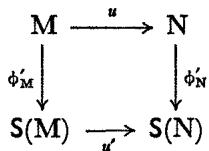
\includegraphics[keepaspectratio]{images/part003_0f38c769.jpg}}

是交换的。此外， \(u'\) 是分次代数同态。

\(u'\) 的存在性与唯一性由第 1 号命题 2 应用于交换代数 \(\mathbf{S}(\mathbf{N})\) 和 \(f = \phi_{\mathbf{N}}' \circ u: \mathbf{M} \to \mathbf{S}(\mathbf{N})\) 得出；由于

\[
f (\mathbf {M}) \subset \mathbf {S} ^ {1} (\mathbf {N}) = \mathbf {N},
\]

\(u'\) 是分次代数同态这一事实由第 1 号注记 1 得出。

命题 3 中的同态 \(u'\) 此后将记为 \(S(u)\) 。若 \(P\) 是一个 A-模，且 \(v: N \to P\) 是一个 A-线性映射，则

\[
\mathbf {S} (v \circ u) = \mathbf {S} (v) \circ \mathbf {S} (u)\tag{3}
\]

因为 \(\mathbf{S}(v) \circ \mathbf{S}(u)\) 是使下图交换的代数同态

\pandocbounded{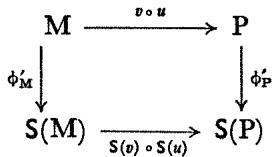
\includegraphics[keepaspectratio]{images/part003_67e6d402.jpg}}

由于 \(\mathbf{S}(\mathbf{M})\) 包含 \(\mathbf{M} = \mathbf{S}^1 (\mathbf{M})\) , \(\mathbf{S}(u)\) 有时称为 \(u\) 到 \(\mathbf{S}(\mathbf{M})\) 的典范扩张。限制 \(\mathbf{S}^n (u): \mathbf{S}^n (\mathbf{M}) \to \mathbf{S}^n (\mathbf{N})\) 满足

\[
\mathsf {S} ^ {n} (u) \left(x _ {1} x _ {2} \dots x _ {n}\right) = u \left(x _ {1}\right) u \left(x _ {2}\right) \dots u \left(x _ {n}\right)
\]

其中 \(x_{i} \in M\) ，因为 \(\mathbf{S}(u)\) 是一个代数同态且 \(\mathbf{S}^{1}(u) = u\) ；\(\mathbf{S}^{0}(u)\) 在 A 上的限制是恒等映射。注意， \(\mathbf{S}^{n}(u)\) 可以由 \(\mathbf{T}^{n}(u): \mathbf{T}^{n}(\mathbf{M}) \to \mathbf{T}^{n}(\mathbf{N})\) 通过过渡到商得到。

命题4. 若 \(u: \mathbf{M} \to \mathbf{N}\) 是满射 A-线性映射，则同态 \(\mathbf{S}(u): \mathbf{S}(\mathbf{M}) \to \mathbf{S}(\mathbf{N})\) 是满射的，且其核是 \(\mathbf{S}(\mathbf{M})\) 的由核 \(\mathbf{P} \subset \mathbf{M} \subset \mathbf{S}(\mathbf{M})\) （即 \(u\) 的核）生成的理想。

我们记 \(v = \mathsf{T}(u) \colon \mathsf{T}(\mathbf{M}) \to \mathsf{T}(\mathbf{N})\) ；我们知道（§5，第 2 号，命题 3） \(v\) 是满射的，因此由定义可知 \(v(\mathfrak{J}_{\mathbf{M}}') = \mathfrak{J}_{\mathbf{N}}'\) ；若 \(\Re\) 是 \(v\) 的核，则 \(v^{-1}(\mathfrak{J}_{\mathbf{N}}') = \Re + \mathfrak{J}_{\mathbf{M}}'\) 。由于 \(\mathsf{S}(u) \colon \mathsf{T}(\mathbf{M}) / \mathfrak{J}_{\mathbf{M}}' \to \mathsf{T}(\mathbf{N}) / \mathfrak{J}_{\mathbf{N}}'\) 是由 \(v\) 过渡到商而得到的，它是一个满射同态，其核为 \(\Re' = (\Re + \mathfrak{J}_{\mathbf{M}}') / \mathfrak{J}_{\mathbf{M}}'\) 。由于 \(\Re\) 由核 \(\mathbf{P}\) （即 \(u\) 的核）生成（§5，第 2 号），\(\Re'\) 亦然。

若 \(u: \mathbf{M} \to \mathbf{N}\) 是单射线性映射，\(\mathbf{S}(\mathbf{u})\) 并不总是单射映射（练习1）。然而，当 \(u\) 是使 \(u(\mathbf{M})\) 为 \(\mathbf{N}\) 中直因子的单射时，它是单射的，且此时 \(\mathbf{S}(u)\) 的像（同构于 \(\mathbf{S}(\mathbf{M})\) ）是 \(\mathbf{S}(\mathbf{N})\) 的一个直因子；其证明与关于 \(\mathbf{T}(u)\) 的类似断言（ \(\S 5\) ，第 2 号）的证明相同，只需把 \(\mathbf{T}\) 换为 \(\mathbf{S}\) 。

命题5. 设N和P是A-模M的两个子模，使得它们的和 \(N + P\) 是M中的直因子，且它们的交集 \(N \cap P\) 是N和P中的直因子。则同态 \(\mathsf{S}(\mathsf{N}) \to \mathsf{S}(\mathsf{M}), \mathsf{S}(\mathsf{P}) \to \mathsf{S}(\mathsf{M})\) 和

\[
\mathbf {S} (\mathbf {N} \cap \mathbf {P}) \rightarrow \mathbf {S} (\mathbf {M}),
\]

（即典范单射的典范扩张）都是单射的；如果 \(\mathbf{S}(\mathbf{N})\) , \(\mathbf{S}(\mathbf{P})\) 和 \(\mathbf{S}(\mathbf{N} \cap \mathbf{P})\) 通过这些同态被等同于 \(\mathbf{S}(\mathbf{M})\) 的子代数，则

\[
\mathbf {S} (\mathbf {N} \cap \mathbf {P}) = \mathbf {S} (\mathbf {N}) \cap \mathbf {S} (\mathbf {P}).\tag{4}
\]

证明归结为 §5，第 2 号，命题 4 的证明，只需通篇把 T 换为 S。当A是域时，命题5的假设对M的任意子模N、P总是成立。

推论。设K是一个交换域，M是K上的一个向量空间。对于每一个元素 \(z \in \mathbb{S}(\mathbf{M})\) 存在 M 的一个最小向量子空间 N，使得 \(z \in \mathbb{S}(\mathbf{N})\) 且N是有限维的。

证明的推导源自 §5，第 2 号，命题 4 的推论，只需通篇把 T 换为 S。

N 称为 M 的与 z 相关联的向量子空间。

\subsection{模的 n 次对称幂与对称多重线性映射}

设 X, Y 为两个集合，n 为整数 \(\geqslant1\) 。从 \(X^{n}\) 到 Y 的对称映射是指任意满足以下条件的映射 \(f: X^{n} \to Y\) ：对于每个置换 \(\sigma \in S_{n}\) 以及每个元素 \((x_{i}) \in X^{n}\) ，

\[
f (x _ {\sigma (1)}, x _ {\sigma (2)}, \dots , x _ {\sigma (n)}) = f (x _ {1}, x _ {2}, \dots , x _ {n}).\tag{5}
\]

由于交换两个相邻整数的对换生成群 \(\mathfrak{S}_n\) （I，§ 5，第 7 号），只需条件（5）对 \(\sigma\) 为这样一个对换的情形成立即可。

当 Y 是交换环 A 上的模时，显然从 \(X^{n}\) 到 Y 的对称映射的集合是 A-模 \(Y^{X^{n}}\) （由所有从 \(X^{n}\) 到 Y 的映射组成）的一个子模。

命题6. 设 A 是一个交换环，M 和 N 是两个 A-模。如果对每个 A-线性映射 \(g: \mathbf{S}^n(\mathbf{M}) \to \mathbf{N} (n \geqslant 1)\) 令其对应 n-线性映射

\[
\left(x _ {1}, x _ {2}, \dots , x _ {n}\right) \mapsto g \left(x _ {1} x _ {2} \dots x _ {n}\right)\tag{6}
\]

（其中右端的乘积取在代数 \(\mathbf{S}(\mathbf{M})\) 中），则得到 A-模 \(\operatorname{Hom}_{\mathbf{A}}(\mathbf{S}^{n}(\mathbf{M}), \mathbf{N})\) 到由对称 \(n\) -线性映射（从 \(\mathbf{M}^{n}\) 到 \(\mathbf{N}\) ）组成的 A-模上的一个双射 A-线性映射。

回忆（II，§3，第9号），存在从 A-模 \(\operatorname{Hom}_{\mathbf{A}}(\mathbb{T}^{n}(\mathbf{M}), \mathbf{N})\) 到 A-模 \(\mathcal{L}_{n}(\mathbf{M}, \ldots, \mathbf{M}; \mathbf{N})\) （由所有 \(n\) -线性映射（从 \(\mathbf{M}^{n}\) 到 \(\mathbf{N}\) ）组成）上的典范双射，它是通过把每个 A-线性映射 \(f: \mathbb{T}^{n}(\mathbf{M}) \to \mathbf{N}\) 对应到 \(n\) -线性映射而得到的

\[
\bar {f} \colon (x _ {1}, x _ {2}, \dots , x _ {n}) \mapsto f (x _ {1} \otimes x _ {2} \otimes \dots \otimes x _ {n}).\tag{7}
\]

另一方面，A-线性映射 \(g \colon \mathbb{S}^n(\mathbf{M}) \to \mathbf{N}\) 一一对应于满足以下条件的 A-线性映射 \(f \colon \mathbb{T}^n(\mathbf{M}) \to \mathbf{N}\) ：\(f\) 在 \(\mathfrak{J}_n'\) 上为零；对应方式是把 \(g\) 对应到映射 \(f = g \circ p_n\) ，其中

\[
p _ {n} \colon \mathbf {T} ^ {n} (\mathbf {M}) \rightarrow \mathbf {S} ^ {n} (\mathbf {M}) = \mathbf {T} ^ {n} (\mathbf {M}) / \mathfrak {J} _ {n} ^ {\prime}
\]

是典范同态（II，§ 2，第 1 号，定理 1）。但由于 \(\mathfrak{J}_n'\) 是形如

\[
\left(u _ {1} \otimes u _ {2} \otimes \dots \otimes u _ {p}\right) \otimes (x \otimes y - y \otimes x) \otimes \left(v _ {1} \otimes \dots \otimes v _ {n - p - 2}\right)
\]

\((x, y, u_{i}, v_{j} \text{ in } \mathbf{M})\) 的元素的线性组合，故说函数 f 具有形式 \(g \circ p_{n}\) 就意味着相应的 n-线性函数 \(\bar{f}\) 满足关系

\[
\bar {f} (u _ {1}, \dots , u _ {p}, x, y, v _ {1}, \dots , v _ {n - p - 2}) = \bar {f} (u _ {1}, \dots , u _ {p}, y, x, v _ {1}, \dots , v _ {n - p - 2});
\]

换言之，根据上文所见，这意味着 \(\bar{f}\) 是对称的；由此得到命题，同时考虑到以下事实：

\[
p _ {n} (x _ {1} \otimes x _ {2} \otimes \dots \otimes x _ {n}) = x _ {1} x _ {2} \dots x _ {n}
\]

（其中 \(x_{i} \in M\) ）。

A-模 \(\mathbf{S}^{n}(\mathbf{M})\) 称为 M 的第 n 次对称幂。对于每个 A-模同态 \(u: M \to N\) ，映射 \(\mathbf{S}^{n}(u): \mathbf{S}^{n}(\mathbf{M}) \to \mathbf{S}^{n}(\mathbf{N})\) （它与 \(\mathbf{S}(u)\) 在 \(\mathbf{S}^{n}(\mathbf{M})\) 上相一致）称为 u 的第 n 次对称幂。

注记。设 \(\sigma\) 是 \(\mathfrak{S}_n\) 中的一个置换；由于映射

\[
\left(x _ {1}, x _ {2}, \dots , x _ {n}\right) \mapsto x _ {\sigma^ {- 1} (1)} \otimes x _ {\sigma^ {- 1} (2)} \otimes \dots \otimes x _ {\sigma^ {- 1} (n)}
\]

（从 \(\mathbf{M}^n\) 到 \(\mathbf{T}^n (\mathbf{M})\) ）是 A-多重线性的，它可以唯一地写成

\[
(x _ {1}, \dots , x _ {n}) \mapsto u _ {\sigma} (x _ {1} \otimes x _ {2} \otimes \dots \otimes x _ {n}),
\]

（其中 \(u_{\sigma}\) 是 A-模 \(\mathsf{T}^n(\mathbf{M})\) 的一个自同态，也记作 \(z \mapsto \sigma. z\) 。显然，若 \(\sigma\) 是 \(\mathfrak{S}_n\) 的单位元，则 \(u_{\sigma}\) 是恒等映射；另一方面，写出 \(y_i = x_{\sigma^{-1}(i)}\) ，我们得到：对每个置换 \(\tau \in \mathfrak{S}_n, y_{\tau^{-1}(i)} = x_{\sigma^{-1}(\tau^{-1}(i))}\) ，因此 \(\tau. (\sigma. z) = (\tau \sigma). z\) ；换言之，A-模 \(\mathsf{T}^n(\mathbf{M})\) 是一个左 \(\mathfrak{S}_n\text{-set}\) （运算为 \((\sigma, z) \mapsto \sigma. z\) ，I，§ 5，第 1 号）。 \(\mathsf{T}^n(\mathbf{M})\) 中使得 \(\sigma. z = z\) （对所有 \(\sigma \in \mathfrak{S}_n\) ）的元素称为 \(n\) 阶（反变）对称张量；它们构成 \(\mathsf{S}_n'(\mathbf{M})\) ，即 \(\mathsf{T}^n(\mathbf{M})\) 的一个子 A-模。

对所有 \(z \in \mathbf{T}^n(\mathbf{M})\) ，我们记 \(s.z = \sum_{\sigma \in \mathfrak{S}_n} \sigma.z\) ，并称 \(s.z\) 为张量 \(z\) 的对称化；显然 \(s.z\) 是对称张量，因此 \(z \mapsto s.z\) 是 \(\mathbf{T}^n(\mathbf{M})\) 的自同态，其像 \(\mathbf{S}_n''(\mathbf{M})\) 包含于 \(\mathbf{S}_n'(\mathbf{M})\) ；一般地， \(\mathbf{S}_n''(\mathbf{M}) \neq \mathbf{S}_n'( \mathbf{M})\) （习题5）。若 \(z\) 是对称张量，则 \(s.z = n!z\) ；由此可知，当 \(n!\) 在 \(\mathbf{A}\) 中可逆时，自同态 \(z \mapsto (n!)^{-1}s.z\) 是 \(\mathbf{T}^n(\mathbf{M})\) 的投影算子（II，§1，第8号），其像为 \(\mathbf{S}_n'(\mathbf{M}) = \mathbf{S}_n''(\mathbf{M})\) ；此外，这个投影算子的核恰好是 \(\mathfrak{J}_n'\) 。因为，显然 \(\sigma(\mathfrak{J}_n') \subset \mathfrak{J}_n'\) 对所有 \(\sigma \in \mathfrak{S}_n\) 成立，且 \(\mathfrak{J}_n'\) 按定义由形如 \(z - \rho.z\) 的张量生成，其中 \(\rho\) 是交换 {[}1, n{]} 中两个相邻数字的对换；此外，若 \(\sigma, \tau\) 是 \(\mathfrak{S}_n\) 中的两个置换，则 \(z - (\sigma\tau).z = z - \sigma.z + \sigma.(z - \tau.z)\) ，由此可得（因为 \(\mathfrak{S}_n\) 中的每个置换都是交换两个相邻数字的对换之积） \(z - \sigma.z \in \mathfrak{J}_n'\) 对所有 \(z \in \mathbf{T}^n(\mathbf{M})\) 和 \(\sigma \in \mathfrak{S}_n\) 成立。因此（始终假设 \(n!\) 在 \(\mathbf{A}\) 中可逆），可见 \(z - (n!)^{-1}s.z = \sum_{\sigma \in \mathfrak{S}_n}(n!)^{-1}(z - \sigma.z) \in \mathfrak{J}_n'\) 对所有 \(z \in \mathbf{T}^n(\mathbf{M})\) 成立，这就证明了我们的断言。

当 \(n!\) 在A中可逆时，子模 \(S_n'(M)\) 和 \(\mathfrak{S}_n'\) （ \(T^n(M)\) 中的）因此是互补的，并且典范同态在 \(S_n'(M)\) 上的限制（该典范同态即 \(T^n(M) \to S^n(M) = T^n(M)/\mathfrak{J}_n'\) ）是一个 A-模同构，这使我们在所考虑的情形下可以把 \(n\) 阶对称张量与 M 的第 \(n\) 次对称幂的元素等同起来。但请注意，这种等同与乘法不相容：两个对称张量在 \(T(M)\) 中的乘积一般不是对称的，因此其在 \(S(M)\) 中的像并不是所考虑的对称张量的像的乘积。

\subsection{标量环的扩张}

设 A, A' 为两个交换环， \(\rho: A \to A'\) 为一个环同态，M 为 A-模，M' 为 A'-模，且 \(f: M \to M'\) 为（相对于 \(\rho\) ）从 M 到 M' 的 A-同态。复合映射 \(M \xrightarrow{f} M' \xrightarrow{\phi_{M'}'} S_{A'}(M')\) 是 M 到交换代数 \(\rho_*(S_A(M'))\) 的 A-线性映射；则存在（第 1 号，命题 2）唯一的一个 A-代数同态 \(f': S_A(M) \to S_{A'}(M')\) 使图表交换

\[
\begin{array}{c} \mathrm{M} \xrightarrow {f} \mathrm{M} ^ {\prime} \\ \phi_ {\mathrm{M}} ^ {\prime} \Biggl \downarrow \\ \mathrm{S} _ {\mathrm{A}} (\mathrm{M}) \xrightarrow [ f ^ {\prime} ]{} \mathrm{S} _ {\mathrm{A} ^ {\prime}} (\mathrm{M} ^ {\prime}) \end{array}\tag{8}
\]

由此立即得出，如果 \(\sigma: A' \to A''\) 是另一个环同态， \(M''\) 是一个 \(A''\) -模， \(g: M' \to M''\) 是一个 \(A'\) -同态（相对于 \(\sigma\) ），且 \(g': S_{A'}(M') \to S_{A''}(M'')\) 是相应的 \(A'\) -代数同态，则复合 \(A\) -代数同态

\[
\mathrm{S} _ {\mathrm{A}} (\mathrm{M}) \xrightarrow {f ^ {\prime}} \mathrm{S} _ {\mathrm{A} ^ {\prime}} \left(\mathrm{M} ^ {\prime}\right) \xrightarrow {g ^ {\prime}} \mathrm{S} _ {\mathrm{A} ^ {\prime \prime}} \left(\mathrm{M} ^ {\prime \prime}\right)\tag{9}
\]

对应于复合 A-同态 \(g \circ f: \mathbf{M} \to \mathbf{M}''\) （相对于 \(\sigma \circ \rho\) ）。

命题 7. 设 A，B 为两个交换环， \(\rho: \mathbf{A} \to \mathbf{B}\) 为一个环同态，且 M 是一个 A-模。典范扩张

\[
\psi \colon \mathbf {S} _ {\mathbf {B}} (\mathbf {B} \otimes_ {\mathbf {A}} \mathbf {M}) \rightarrow \mathbf {B} \otimes_ {\mathbf {A}} \mathbf {S} _ {\mathbf {A}} (\mathbf {M})
\]

B-线性映射 \(1_{B} \otimes \phi_{M}'\) : \(B \otimes_{A} M \to B \otimes_{A} S_{A}(M)\) 的典范扩张是一个分次 B-代数同构。

证明由 § 5，第 3 号，命题 5 的证明导出，只需将 T 换为 S 并将 \(\phi_{\mathbf{M}}\) 换为 \(\phi_{\mathbf{M}}^{\prime}\) 。

\subsection{对称代数的直接极限}

设 \((\mathbf{A}_{\alpha},\phi_{\beta \alpha})\) 为交换环的一个有向正向系统， \((\mathbf{M}_{\alpha},f_{\beta \alpha})\) 为一个由 \(\mathbf{A}_{\alpha}\) -模构成的正向系统， \(\mathbf{A} = \varinjlim \mathbf{A}_{\alpha}\) 和 \(\mathbf{M} = \varinjlim \mathbf{M}_{\alpha}\) 。对于 \(\alpha \leqslant \beta\) ，我们从 \(\mathbf{A}_{\alpha}\) -同态 \(f_{\beta \alpha}: \mathbf{M}_{\alpha} \to \mathbf{M}_{\beta}\) 典范地导出一个 \(\mathbf{A}_{\alpha}\) -代数同态（第 4 号，公式 (8)） \(f_{\beta \alpha}': \mathbf{S}_{\mathbf{A}_{\alpha}}(\mathbf{M}_{\alpha}) \to \mathbf{S}_{\mathbf{A}_{\beta}}(\mathbf{M}_{\beta})\) ，并由 (9)（第 4 号）可知 \((\mathbf{S}_{\mathbf{A}_{\alpha}}(\mathbf{M}_{\alpha}), f_{\beta \alpha}')\) 是一个由 \(\mathbf{A}_{\alpha}\) -代数构成的正向系统。另一方面，设 \(f_{\alpha}: \mathbf{M}_{\alpha} \to \mathbf{M}\) 为典范 A-同态；我们（由第 4 号，公式 (8)）导出一个 \(\mathbf{A}_{\alpha}\) -代数同态

\[
f _ {\alpha} ^ {\prime}: \mathrm{S} _ {\mathrm{A} _ {\alpha}} (\mathbf {M} _ {\alpha}) \rightarrow \mathrm{S} _ {\mathrm{A}} (\mathbf {M})
\]

并且由 (9) 也可知诸 \(f_{\alpha}'\) 构成一个由 \(A_{\alpha}\) -同态构成的正向系统。

命题8. A-同态 \(f' = \varinjlim f_{\alpha}' \colon \varinjlim S_{A_{\alpha}}(M_{\alpha}) \to S_{A}(M)\) 是一个分次代数同构。

证明与 § 5，第 5 号，命题 6 的证明相同，只需通篇将 T 换为 S 并将 \(\phi\) 换为 \(\phi'\) ，且注意到交换代数的正向极限是交换的。

\subsection{直和的对称代数。自由模的对称代数。分次模的对称代数}

设 A 为一个交换环， \(M = \bigoplus_{\lambda \in L} M_{\lambda}\) 为一族 A-模的直和， \(j_{\lambda}: M_{\lambda} \to M\) 为典范单射；我们导出一个 A-代数同态 \(\mathsf{S}(j_{\lambda}): \mathsf{S}(\mathsf{M}_{\lambda}) \to \mathsf{S}(\mathsf{M})\) 。由于 \(\mathsf{S}(\mathsf{M})\) 是交换的，§ 4，第 5 号，命题 8 可应用于诸同态 \(\mathsf{S}(j_{\lambda})\) ，因此存在唯一的代数同态

\[
g \colon \bigotimes_ {\lambda \in L} \mathbf {S} (\mathbf {M} _ {\lambda}) \rightarrow \mathbf {S} (\mathbf {M})\tag{10}
\]

（也记作 \(g_{\mathbf{M}}\) ）使得 \(\mathbf{S}(j_{\lambda}) = g \circ f_{\lambda}\) （对所有 \(\lambda \in \mathbf{L}\) ），其中

\[
f _ {\lambda} \colon \mathbf {S} (\mathbf {M} _ {\lambda}) \rightarrow \bigotimes_ {\lambda \in \mathbf {L}} \mathbf {S} (\mathbf {M} _ {\lambda})
\]

表示典范同态。

命题 9. 典范同态 \(g\) （公式 (10)）是一个分次代数同构（参见 § 4，第 8 号，注 1）。

为了证明 \(g\) 是双射的，我们定义一个代数同态

\begin{enumerate}
\def\labelenumi{(\arabic{enumi})}
\setcounter{enumi}{10}
\tightlist
\item
\end{enumerate}

\[
h \colon \mathbf {S} (\mathbf {M}) \rightarrow \bigotimes_ {\lambda \in L} \mathbf {S} (\mathbf {M} _ {\lambda})
\]

使得 \(g \circ h\) 和 \(h \circ g\) 分别是 \(\mathbf{S}(\mathbf{M})\) 和 \(\bigotimes_{\lambda \in \mathbf{L}} \mathbf{S}(\mathbf{M}_{\lambda})\) 上的恒等映射。对于每个 \(\lambda \in \mathbf{L}\) ，设 \(u_{\lambda}\) 为复合线性映射

\[
\mathbf {M} _ {\lambda} \xrightarrow {\phi_ {\mathrm{M} _ {\lambda}} ^ {\prime}} \mathbf {S} (\mathbf {M} _ {\lambda}) \xrightarrow {f _ {\lambda}} \bigotimes_ {\lambda \in L} \mathbf {S} (\mathbf {M} _ {\lambda}).
\]

存在唯一的 A-线性映射 \(u: \mathbf{M} \to \bigotimes_{\lambda \in L} \mathbf{S}(\mathbf{M}_{\lambda})\) ，使得 \(u \circ j_{\lambda} = u_{\lambda}\) （对所有 \(\lambda \in L\) ）。由于诸 \(\mathbf{S}(\mathbf{M}_{\lambda})\) 是交换的，它们的张量积也是交换的（§ 4，第 5 号），因此（第 1 号，命题 2）存在唯一的代数同态 \(h: \mathbf{S}(\mathbf{M}) \to \bigotimes_{\lambda \in L} \mathbf{S}(\mathbf{M}_{\lambda})\) ，使得 \(h \circ \phi_{\mathbf{M}}' = u\) ；另一方面，显然 \(u(\mathbf{M})\) 包含于分次代数 \(\bigotimes_{\lambda \in L} \mathbf{S}(\mathbf{M}_{\lambda})\) 的次数为 1 的元素所构成的子模中，因此 \(h\) 是一个分次代数同态。对于 \(x_{\lambda} \in \mathbf{M}_{\lambda}\) ，

\[
h \left(g \left(u _ {\lambda} \left(x _ {\lambda}\right)\right)\right) = h \left(g \left(f _ {\lambda} \left(\phi_ {M _ {\lambda}} ^ {\prime} \left(x _ {\lambda}\right)\right)\right)\right) = h \left(S \left(j _ {\lambda}\right) \left(\phi_ {M _ {\lambda}} ^ {\prime} \left(x _ {\lambda}\right)\right)\right) = h \left(\phi_ {M} ^ {\prime} \left(j _ {\lambda} \left(x _ {\lambda}\right)\right)\right) = u _ {\lambda} \left(x _ {\lambda}\right);
\]

由于诸 \(u_{\lambda}(x_{\lambda})\) 生成代数 \(\bigotimes_{\lambda \in L} S(M_{\lambda})\) （§ 4，第 5 号，命题 8）， \(h \circ g\) 当然是恒等映射。类似地，

\[
g \left(h \left(\phi_ {\mathrm{M}} ^ {\prime} \left(j _ {\lambda} \left(x _ {\lambda}\right)\right)\right)\right) = g \left(u _ {\lambda} \left(x _ {\lambda}\right)\right) = g \left(f _ {\lambda} \left(\phi_ {\mathrm{M} _ {\lambda}} ^ {\prime} \left(x _ {\lambda}\right)\right)\right) = \mathrm{S} \left(j _ {\lambda}\right) \left(\phi_ {\mathrm{M} _ {\lambda}} ^ {\prime} \left(x _ {\lambda}\right)\right) = \phi_ {\mathrm{M}} ^ {\prime} \left(j _ {\lambda} \left(x _ {\lambda}\right)\right)
\]

并且，由于诸元素 \(\phi_{\mathbf{M}}^{\prime}(j_{\lambda}(x_{\lambda}))\) 生成代数 \(\mathbf{S}(\mathbf{M})\) ， \(g \circ h\) 当然是恒等映射。

注记 (1) 设 \(\mathbf{N} = \bigoplus_{\lambda \in L} \mathbf{N}_{\lambda}\) 是另一族以 \(L\) 为指标集的 A-模的直和，并且对所有 \(\lambda \in L\) ，设 \(v_{\lambda}: \mathbf{M}_{\lambda} \to \mathbf{N}_{\lambda}\) 是一个 A-线性映射，由此存在一个 A-线性映射 \(v = \bigoplus_{\lambda} v_{\lambda}: \mathbf{M} \to \mathbf{N}\) (II，§1，第6号，命题6)。则图表

\[
\begin{array}{c} \bigotimes_ {\lambda \in L} S (M _ {\lambda}) \xrightarrow {g _ {M}} S (M) \\ \bigoplus_ {\lambda \in L} S (v _ {\lambda}) \Biggl \downarrow \qquad \qquad \qquad \qquad \qquad \qquad \qquad \qquad \qquad \Biggl \downarrow S (v) \\ \bigotimes_ {\lambda \in L} S (N _ {\lambda}) \xrightarrow {g _ {N}} S (N) \end{array}
\]

是交换的，这由定义直接得出（§ 4，第 5 号，命题 8 的推论）。

\(\bigotimes_{\lambda \in L} \mathbf{S}(\mathbf{M}_{\lambda})\) 中与 \(\mathbf{S}^n(\mathbf{M})\) 通过同构 \(g\) 等同起来的那个 A-子模可以更精确地描述。对于每个有限子集 \(J\) （ \(L\) 中的），我们记 \(\mathbf{E}_J = \bigotimes_{\lambda \in J} \mathbf{S}(\mathbf{M}_{\lambda})\) ，使得 \(\bigotimes_{\lambda \in L} \mathbf{S}(\mathbf{M}_{\lambda}) = \varinjlim \mathbf{E}_J\) （相对于有向集 \(\mathfrak{F}(\mathrm{L})\) ，即由 \(\mathbf{L}\) 的有限子集组成的集，根据定义，§ 4，第 5 号）。对于每个族 \(\nu = (n_{\lambda}) \in \mathbf{N}^{(\mathbf{L})}\) （因而具有有限支撑）满足 \(\sum_{\lambda \in \mathbf{L}} n_{\lambda} = n\) ，以及每个有限子集 \(\mathbf{J}\) （ \(\mathbf{L}\) 中的）——包含族 \(\nu\) 的支集——，我们记

\[
\mathbf {S} ^ {\mathrm{J}, \nu} (\mathbf {M}) = \bigotimes_ {\lambda \in J} \mathbf {S} ^ {n _ {\lambda}} (\mathbf {M} _ {\lambda})\tag{12}
\]

使得子模 \(E_{J,n}\) （由次数为 n 的、属于 \(E_{J}\) 的元素组成）是诸 \(S^{J,v}(M)\) 的直和，遍历所有支集包含于 J 且满足 \(\sum_{\lambda\in L}n_{\lambda}=n\) 的族 v（ \(\S4\) ，第7号，命题10和 \(\S4\) ，第8号）。作为约定，我们对支集不包含在 J 中的族 v 写 \(S^{J,v}(M)=\{0\}\) ；那么 \(E_{J,n}\) 也可以写成所有 \(S^{J,v}(M)\) 的直和，其中 v 遍历集合 \(H_{n}\) ，即所有族 \(v=(n_{\lambda})_{\lambda\in L}\) 中满足 \(\sum_{\lambda\in L}n_{\lambda}=n\) 的那些族组成的集合。由于 \(S^{0}(M_{\lambda})\) 与 A 等同，显然还有：对于 L 的两个有限子集 \(J\subset J'\) 以及一个支集包含于 J 中的族 v，典范映射 \(S^{J,v}(M)\to S^{J',v}(M)\) （典范映射 \(E_{J}\to E_{J'}\) 在 \(S^{J,v}(M)\) 上的限制）是双射。如果对所有 \(v\in H_{n}\) 我们写

\[
\mathbf {S} ^ {\nu} (\mathbf {M}) = \varinjlim \mathbf {S} ^ {\mathrm{J}, \nu} (\mathbf {M})\tag{13}
\]

由此可见，结合II，§6，第2号，命题5：

推论。A-模 \(\mathbf{S}^n (\mathbf{M})\) 是 \(\bigotimes_{\lambda \in \mathbf{L}}\mathbf{S}(\mathbf{M}_{\lambda})\) 的这样一个子模在同构 (10) 下的像：该子模是诸子模 \(\mathbf{S}^{\nu}(\mathbf{M})\) 的直和，遍历所有族 \(\nu = (n_{\lambda})\in \mathbf{N}^{(L)}\) （满足 \(\sum_{\lambda \in \mathbf{L}}n_{\lambda} = n\) ）；若 \(\mathbf{J}\) 是 \(\nu\) 的支集，则 \(\mathbf{S}^{\nu}(\mathbf{M})\) 典范同构于 \(\bigotimes_{\lambda \in \mathbf{J}}\mathrm{S}^{n_{\lambda}}(\mathbf{M}_{\lambda})\) 。

一般地， \(\mathbf{S}^{\nu}(\mathbf{M}),\bigotimes_{\lambda \in J}\mathbf{S}^{n_{\lambda}}(\mathbf{M}_{\lambda})\) 以及它们在 \(\mathbf{S}^n (\mathbf{M})\) 中的像被等同起来。

定理 1. 设 A 是一个交换环，M 是一个以 \((e_{\lambda})_{\lambda \in L}\) 为基的自由 A-模。对于每个具有有限支撑的映射 \(\alpha: \mathbf{L} \to \mathbf{N}\) ，我们记

\[
e ^ {\alpha} = \prod_ {\lambda \in L} e _ {\lambda} ^ {\alpha (\lambda)}\tag{14}
\]

（乘积取在交换代数 \(\mathbf{S}(\mathbf{M})\) 中）。然后，当 \(\alpha\) 遍历集合 \(\mathbf{N}^{(L)}\) （由从 \(\mathbf{L}\) 到 \(\mathbf{N}\) 的具有有限支撑的映射组成）时，诸 \(e^{\alpha}\) 构成 A-模 \(\mathbf{S}(\mathbf{M})\) 的一组基。

由于 M 是诸 \(M_{\lambda} = Ae_{\lambda}\) 的直和，只需在 L 约化为单个元素时证明该定理，然后应用命题 9 即可。但当 M = Ae（e 为自由元素）时， \(x \otimes y - y \otimes x = 0\) 对所有 x, y 属于 M 成立；理想 \(J'\) 因此为零，从而 \(\mathsf{T}(\mathsf{A}e) = \mathsf{S}(\mathsf{A}e)\) ，于是定理由 § 5，第 5 号，定理 1 得出。

基(14)的乘法表由下式给出

\[
e ^ {\alpha} e ^ {\beta} = e ^ {\alpha + \beta}\tag{15}
\]

（其中 \(\alpha + \beta\) 是从 L 到 N 的映射 \(\lambda \mapsto \alpha(\lambda) + \beta(\lambda)\) 。换言之，S(M) 的基 \((e^{\alpha})\) 连同乘法法则 (15) 典范同构于由 L 导出的自由交换幺半群 \(\mathbf{N}^{(L)}\) ；由此得出（§ 2，第 9 号）：基的指标集为 L 的自由模 M 的对称代数 S(M) 典范同构于多项式代数 A{[}(X \(_{\lambda}\) ) \(_{\lambda \in L}\) {]}，典范同构通过将 \(e_{\lambda}\) 映为 X \(_{\lambda}\) 而得到。特别地（§ 2，第 7 号，命题 7），对于每个从 L 到交换 A-代数 E 中的映射 \(f\colon\) L \(\to\) E ，存在唯一的 A-代数同态 \(\bar{f}\colon\) S(M) \(\to\) E 使得 \(\bar{f}(e_{\lambda}) = f(\lambda)\) 。

注记（2）。上述结果同样可以作为多项式代数和对称代数的泛性质的一个推论而得到，同时考虑到II，§1，第11号，命题17的推论3。

推论。若M是投射A-模，则S(M)是投射A-模。

证明与 § 5，第 5 号，定理 1 的推论的证明相同，只需将 T 换为 S。

命题 10. 设 \(\Delta\) 是一个交换幺半群， \(\mathbf{M}\) 是一个 \(\Delta\) 型分次 A-模， \((\mathbf{M}_{\alpha})_{\alpha \in \Delta}\) 是它的分次。对于每个有序对 \((\alpha, n) \in \Delta \times \mathbf{N}\) ，设 \(\mathbf{S}^{\alpha, n}(\mathbf{M})\) 是 \(\mathbf{S}^n(\mathbf{M})\) 的这样一个子模：诸子模 \(\bigotimes_{\lambda \in J} \mathbf{S}^{n_{\lambda}}(\mathbf{M}_{\alpha_{\lambda}})\) 的直和，其中 \((n_{\lambda})_{\lambda \in L}\) 遍历 \(\geqslant 0\) 的整数族中满足 \(\sum_{\lambda \in L} n_{\lambda} = n, J\) 是其支集的那些族组成的集合，且对每个 \((n_{\lambda})\) , \((\alpha_{\lambda})_{\lambda \in J}\) 遍历 \(\Delta^J\) 的族中满足 \(\sum_{\lambda \in J} \alpha_{\lambda} = \alpha\) 的那些族组成的集合。则 \((\mathbf{S}^{\alpha, n}(\mathbf{M}))_{(\alpha, n) \in \Delta \times \mathbf{N}}\) 是唯一的 \(\Delta \times \mathbf{N}\) 型分次，它与 \(\mathbf{S}(\mathbf{M})\) 上的代数结构相容，并且在 \(\mathbf{M} = \mathbf{S}^1(\mathbf{M})\) 上诱导出给定的分次。

\(\mathbf{S}(\mathbf{M})\) 是诸 \(\mathbf{S}^{\alpha,n}(\mathbf{M})\) 的直和这一事实由命题 9 的推论得出；证明的其余部分与 § 5，第 5 号，命题 7 的证明的结尾完全相同。

更特别地假设 \(\Delta = \mathbf{Z}\) ，并给 \(\mathbb{S}(\mathbf{M})\) 赋予总分次（ \(\mathbf{Z}\) 型）（II，§11，第1号），它对应于上面定义的 \(\mathbf{Z} \times \mathbf{N}\) 型（因而也是 \(\mathbf{Z} \times \mathbf{Z}\) 型）分次；在此分次下次数为 \(n \in \mathbf{Z}\) 的齐次元素因此是属于诸 \(\mathbb{S}^{q, m}(\mathbf{M})\) ——对 \(q + m = n\) ——的直和的那些元素。设 \(f\) 是分次 A-模 \(\mathbf{M}\) 到交换分次 A-代数 \(\mathbf{F}\) （ \(\mathbf{Z}\) 型）的 0 次齐次线性映射；则代数同态 \(g: \mathbb{S}(\mathbf{M}) \to \mathbf{F}\) ——它满足 \(f = g \circ \phi_{\mathbf{M}}'\) ——是一个 \(\mathbf{Z}\) 型分次代数同态，这由公式 \(g(x_1 x_2 \ldots x_n) = f(x_1) f(x_2) \ldots f(x_n)\) （对齐次的 \(x_i\) ，属于 \(\mathbf{M}\) ）、关于 \(f\) 的假设以及 \(\mathbf{Z}\) 型分次在 \(\mathbb{S}(\mathbf{M})\) 上的定义得出。

\section{外代数}

\subsection{模的外代数的定义}

定义 1. 设 A 是一个交换环，M 是一个 A-模。M 的外代数，记为 \(\bigwedge (\mathbf{M})\) 或 \(\operatorname {Alt}(\mathbf{M})\) 或 \(\bigwedge_{\mathbf{A}}(\mathbf{M})\) ，是 A 上的这样一个代数：张量代数 \(\mathsf{T}(\mathbf{M})\) 关于双边理想 \(\mathfrak{J}''\) （也记作 \(\mathfrak{J}_{\mathbf{M}}''\) ）——由元素 \(x\otimes x\) （其中 \(x\) 遍历 M）生成——的商代数。

由于理想 \(\mathfrak{J}''\) 由次数为 2 的齐次元素生成，它是一个分次理想（II，§11，第3号，命题2）；我们记 \(\mathfrak{J}_n'' = \mathfrak{J}'' \cap \mathsf{T}^n(\mathbf{M})\) ；代数 \(\bigwedge(\mathbf{M})\) 因此由诸 \(\bigwedge^n(\mathbf{M}) = \mathsf{T}^n(\mathbf{M}) / \mathfrak{J}_n''\) 组成的（称为典范的）分次进行分次。则 \(\mathfrak{J}_0'' = \mathfrak{J}_1'' = \{0\}\) ，因此 \(\bigwedge^0(\mathbf{M})\) 与 A 等同，且 \(\bigwedge^1(\mathbf{M})\) 与 \(\mathsf{T}^1(\mathbf{M}) = \mathbf{M}\) 等同；在下文中我们始终作这些等同，且典范单射 \(\mathbf{M} \to \bigwedge(\mathbf{M})\) 将记作 \(\phi''\) 或 \(\phi_{\mathbf{M}}''\) 。

命题 1. 设 E 为一个 A-代数，且 \(f: \mathbf{M} \to \mathbf{E}\) 为一个满足如下条件的 A-线性映射：

\[
(f (x)) ^ {2} = 0 \quad \text { for all } x \in \mathbf {M}.\tag{1}
\]

存在唯一的 A-代数同态 \(g: \bigwedge(\mathbf{M}) \to \mathbf{E}\) ，使得 \(f = g \circ \phi''\) 。

换言之， \((\bigwedge (\mathbf{M}),\phi '')\) 是泛映射问题（集合论，IV，§3，第1号）的一个解，其中 \(\Sigma\) 是 A-代数结构的类， \(\alpha\) -映射为从 A-模 M 到满足 (1) 的 A-代数的线性映射。

\(g\) 的唯一性由以下事实推出： \(\phi''(\mathbf{M}) = \mathbf{M}\) 生成 \(\bigwedge (\mathbf{M})\) 。为证明 \(g\) 的存在性，我们注意到由 § 5，第 1 号，命题 1，存在一个 A-代数同态 \(g_1: \mathsf{T}(\mathbf{M}) \to \mathbf{E}\) ，使得 \(f = g_1 \circ \phi\) ；我们需要证明 \(g_1\) 在理想 \(\mathfrak{J}''\) 上为零，因为若

\[
p \colon \mathbf {T} (\mathbf {M}) \rightarrow \bigwedge (\mathbf {M}) = \mathbf {T} (\mathbf {M}) / \mathfrak {J} ^ {\prime \prime}
\]

是典范同态，则可写 \(g_1 = g \circ p\) ，其中 \(g: \bigwedge (\mathbf{M}) \to \mathbf{E}\) 是一个代数同态，且结论将由以下事实推出： \(p \circ \phi = \phi''\) 。现在， \(g_1\) 的核是一个双边理想，由 (1) 及关系 \(g_1 \circ \phi = f\) ，它包含元素 \(x \otimes x\) （对 \(x \in \mathbf{M}\) ）。这就完成了证明。

注记. (1) 设 E 为 Z 型分次 A-代数，其分次为 \((\mathbf{E}_{n})\) ，并设线性映射 f（假定满足 (1)）满足

\[
f (\mathbf {M}) \subset \mathbf {E} _ {1}.\tag{2}
\]

则关系 \(g(x_1x_2 \ldots x_p) = f(x_1)f(x_2) \ldots f(x_p)\) （其中 \(x_i \in \mathbf{M}\) ）表明 \(g(\bigwedge^p (\mathbf{M})) \subset \mathrm{E}_p\) （对所有 \(p \geqslant 0\) ），因此 \(g\) 是一个分次代数同态。

\begin{enumerate}
\def\labelenumi{(\arabic{enumi})}
\setcounter{enumi}{1}
\tightlist
\item
  为避免混淆，外代数 \(\bigwedge(\mathbf{M})\) 中两个元素 u, v 的乘积通常记为 \(u \wedge v\) ，并称为 u 与 v 的外积。 \(\bigwedge^{n}(\mathbf{M})\) 的元素因此是形如 \(x_{1} \wedge x_{2} \wedge \cdots \wedge x_{n}\) 的元素之和（其中 \(x_{i} \in M\) ， \(1 \leqslant i \leqslant n\) ），常称为 n-向量。
\end{enumerate}

\subsection{外代数的函子性质}

命题 2. 设 A 是一个交换环，M 和 N 是两个 A-模，u: M → N 是一个 A-线性映射。则存在唯一的 A-代数同态

\[
u ^ {\prime \prime}: \bigwedge (\mathbf {M}) \rightarrow \bigwedge (\mathbf {N})
\]

使得图表

\pandocbounded{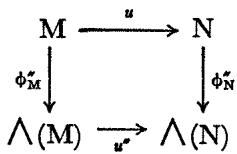
\includegraphics[keepaspectratio]{images/part003_b216bf24.jpg}}

是交换的。此外， \(u''\) 是一个分次代数同态。

\(u''\) 的存在性与唯一性由第 1 号，命题 1 应用于代数 \(\bigwedge(\mathbf{N})\) 和 \(f = \phi_{\mathbf{N}}'' \circ u: \mathbf{M} \to \bigwedge(\mathbf{N})\) 得出；因为 \(f(\mathbf{M}) \subset \mathbf{N}\) ，因此 \(f\) 由 \(\mathfrak{J}_{\mathbf{N}}''\) 的定义满足条件 (1)：由于 \(f(\mathbf{M}) \subset \bigwedge^{1}(\mathbf{N}) = \mathbf{N}\) ，\(u''\) 是分次代数同态这一事实由第 1 号的注记 1 得出。

命题 2 中的同态 \(u''\) 此后将记为 \(\bigwedge(u)\) 。若 P 是一个 A-模且 \(v: \mathbf{N} \to \mathbf{P}\) 是一个 A-线性映射，则

\[
\bigwedge (v \circ u) = \bigwedge (v) \circ \bigwedge (u)\tag{3}
\]

因为 \(\bigwedge(v) \circ \bigwedge(u)\) 是一个代数同态，它使下图交换

\pandocbounded{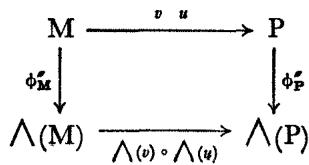
\includegraphics[keepaspectratio]{images/part003_3a522f8d.jpg}}

由于 \(\bigwedge (\mathbf{M})\) 包含 \(\mathbf{M} = \bigwedge^{1}(\mathbf{M}),\bigwedge (u)\) 有时称为 \(u\) 到 \(\bigwedge (\mathbf{M})\) 的典范扩张。限制 \(\bigwedge^n (u):\bigwedge^n (\mathbf{M})\to \bigwedge^n (\mathbf{N})\) 满足

\[
\bigwedge^ {n} (u) (x _ {1} \land x _ {2} \land \dots \land x _ {n}) = u (x _ {1}) \land u (x _ {2}) \land \dots \land u (x _ {n})\tag{4}
\]

（其中 \(x_{i}\in\mathbf{M}\) ），因为 \(\bigwedge(u)\) 是一个代数同态且 \(\bigwedge^{1}(u)=u\) ；限制 \(\bigwedge^{0}(u)\) 在 A 上是恒等映射。注意， \(\bigwedge^{n}(u)\) 是由 \(\mathsf{T}^{n}(u):\mathsf{T}^{n}(\mathbf{M})\to\mathsf{T}^{n}(\mathbf{N})\) 通过过渡到商而得到的。

命题 3. 若 \(u: \mathbf{M} \to \mathbf{N}\) 是满射 A-线性映射，则同态 \(\bigwedge(u): \bigwedge(\mathbf{M}) \to \bigwedge(\mathbf{N})\) 是满射的，且其核为 \(\bigwedge(\mathbf{M})\) 中由核 \(\mathbf{P} \subset \mathbf{M} \subset \bigwedge(\mathbf{M})\) （即 \(u\) 的核）生成的双边理想。

证明由 § 6，第 2 号，命题 4 的证明导出，只需将 S 换为 \(\bigwedge\) 并将 \(\mathfrak{J}'\) 换为 \(\mathfrak{J}''\) 。

若 \(u: \mathbf{M} \to \mathbf{N}\) 是单射线性映射， \(\bigwedge(\mathbf{u})\) 并不总是单射映射（§ 6，练习 3）（然而参见下文第 9 号，命题 12 的推论）。但当 \(u\) 是使得 \(u(\mathbf{M})\) 为 \(\mathbf{N}\) 的直因子的单射时，情况确实如此，且此时 \(\bigwedge(u)\) （同构于 \(\bigwedge(\mathbf{M})\) ）的像是 \(\bigwedge(\mathbf{N})\) 的直因子；其证明与关于 \(\mathbf{T}(u)\) 的类似断言的证明相同（§ 5，第 2 号），只需将 \(\mathbf{T}\) 换为 \(\bigwedge\) 。

命题 4. 设 N 和 P 是 A-模 M 的两个子模，使得它们的和 N + P 是 M 中的直和因子，且它们的交 N ∩ P 是 N 和 P 中的直和因子。则同态 \(\bigwedge(\mathrm{N}) \to \bigwedge(\mathrm{M})\) , \(\bigwedge(\mathrm{P}) \to \bigwedge(\mathrm{M})\) 和 \(\bigwedge(\mathrm{N} \cap \mathrm{P}) \to \bigwedge(\mathrm{M})\) ，即典范单射的典范扩张，是单射；若 \(\bigwedge(\mathrm{N})\) , \(\bigwedge(\mathrm{P})\) 和 \(\bigwedge(\mathrm{N} \cap \mathrm{P})\) 通过这些同态被等同于 \(\bigwedge(\mathrm{M})\) 的子代数，则

\[
\bigwedge (\mathbf {N} \cap \mathbf {P}) = \bigwedge (\mathbf {N}) \cap \bigwedge (\mathbf {P}).\tag{5}
\]

其证明由 § 5，第 2 号，命题 4 的证明导出，只需通篇将 T 换为 \(\bigwedge\) 。当 A 是域时，命题 4 的假设总是被 M 的任意子模 N, P 满足。

推论。设 K 是一个交换域，M 是 K 上的一个向量空间。对每个元素 \(z \in \bigwedge(\mathbf{M})\) ，存在 M 的一个最小向量子空间 N，使得 \(z \in \bigwedge(\mathbf{N})\) 且 N 是有限维的。

证明由 § 5，第 2 号，命题 4 的推论的证明导出，只需通篇将 T 换为 \(\bigwedge\) 。

N 称为 M 的与 \(\bigwedge(\mathbf{M})\) 的元素 z 相关联的向量子空间。
